

\documentclass{article}

\usepackage[margin=1in]{geometry} 
\usepackage{amsmath,amsthm,amssymb,hyperref}
\usepackage{upgreek, mathrsfs, bm}
\usepackage{enumerate}
% \usepackage[inline]{enumitem} % Add inline option for enumerations
\usepackage{mathalpha}
\usepackage{upgreek}
\usepackage{mathrsfs}
\usepackage{amsmath,amsthm,amssymb, mathtools}
\usepackage{yhmath, faktor, dsfont}
\usepackage{academicons, wasysym, marvosym}
\usepackage[scr]{rsfso} 
\usepackage{tikz-cd}
\usepackage[breakable]{tcolorbox}
\usetikzlibrary{decorations.pathmorphing}
\usetikzlibrary{calc, arrows,matrix}
\usepackage{graphicx}
\usepackage{subcaption}

\linespread{1.25}
\def\upint{\mathchoice%
    {\mkern13mu\overline{\vphantom{\intop}\mkern7mu}\mkern-20mu}%
    {\mkern7mu\overline{\vphantom{\intop}\mkern7mu}\mkern-14mu}%
    {\mkern7mu\overline{\vphantom{\intop}\mkern7mu}\mkern-14mu}%
    {\mkern7mu\overline{\vphantom{\intop}\mkern7mu}\mkern-14mu}%
  \int}
  
\def\lowint{\mkern3mu\underline{\vphantom{\intop}\mkern7mu}\mkern-10mu\int}

\newcommand{\N}{\mathbb{N}}
\newcommand{\Z}{\mathbb{Z}}
\newcommand{\Q}{\mathbb{Q}}
\newcommand{\R}{\mathbb{R}}
\newcommand{\C}{\mathbb{C}}
\newcommand{\F}{\mathbb{F}}
\renewcommand{\Pr}{\mathbb{P}}
\newcommand{\E}{\mathbb{E}}
\newcommand{\B}{\mathcal{B}}
\newcommand{\mcC}{\mathcal{C}}
\newcommand{\orbit}{\mathcal{O}}
\renewcommand{\L}{\mathcal{L}}

\newenvironment{theorem}[2][Theorem]{\begin{trivlist}
\item[\hskip \labelsep {\bfseries #1}\hskip \labelsep {\bfseries #2.}]}{\end{trivlist}}
\newenvironment{lemma}[2][Lemma]{\begin{trivlist}
\item[\hskip \labelsep {\bfseries #1}\hskip \labelsep {\bfseries #2.}]}{\end{trivlist}}
\newenvironment{exercise}[2][Exercise]{\begin{trivlist}
\item[\hskip \labelsep {\bfseries #1}\hskip \labelsep {\bfseries #2.}]}{\end{trivlist}}
\newenvironment{problem}[2][Problem]{\begin{trivlist}
\item[\hskip \labelsep {\bfseries #1}\hskip \labelsep {\bfseries #2.}]}{\end{trivlist}}
\newenvironment{question}[2][Question]{\begin{trivlist}
\item[\hskip \labelsep {\bfseries #1}\hskip \labelsep {\bfseries #2.}]}{\end{trivlist}}
\newenvironment{corollary}[2][Corollary]{\begin{trivlist}
\item[\hskip \labelsep {\bfseries #1}\hskip \labelsep {\bfseries #2.}]}{\end{trivlist}}
\newcommand\bigzero{\makebox(0,0){\text{\huge0}}}
\newenvironment{solution}{\begin{proof}[Solution]}{\end{proof}}
\newcommand{\spike}[2]% #1 = size of spike, #2 = centered text
{\bgroup
  \sbox0{#2}%
  \rlap{\usebox0}%
  \hspace{0.5\wd0}%
  \makebox[0pt][c]{\rule[\dimexpr \ht0+1pt]{0.5pt}{#1}}% top spike
  \makebox[0pt][c]{\rule[\dimexpr -\dp0-#1-1pt]{0.5pt}{#1}}% bottom spike
  \hspace{0.5\wd0}%
\egroup}
\renewcommand{\L}{\mathcal{L}}
\newcommand\restr[2]{{% we make the whole thing an ordinary symbol
  \left.\kern-\nulldelimiterspace % automatically resize the bar with \right
  #1 % the function
  \littletaller % pretend it's a little taller at normal size
  \right|_{#2} % this is the delimiter
  }}
\newcommand{\littletaller}{\mathchoice{\vphantom{\big|}}{}{}{}}
\DeclareMathOperator{\vsspan}{span}
\DeclareMathOperator{\image}{im}
\DeclareMathOperator{\nullity}{nullity}
\DeclareMathOperator{\rank}{rank}
\DeclareMathOperator{\ch}{ch}
\DeclareMathOperator{\tr}{tr}
\DeclareMathOperator{\reff}{rref}
\DeclareMathOperator{\Aut}{Aut}
\DeclareMathOperator{\Inn}{Inn}
\DeclareMathOperator{\Char}{char}

\begin{document}

% ------------------------------------------ %
%                 START HERE                  %
% ------------------------------------------ %

\title{Dummit and Foote chap 4 solution} % Replace with appropriate title
\author{Hsin-Wei, Chen\\b12902132@ntu.edu.tw\\} % Replace "Author's Name" with your name

\maketitle
\section*{4.1 Group action and permutation presentation}
Missing exercise number : 5
\begin{problem}{1}\hspace{0.1cm}
    Let $G$ act on the set $A$. Prove that if $a, b \in A$ and for some $b = g \cdot a$ for some $g\in G$, then $G_b = g G_a g^{-1}$. Deduce that if $G$ acts transitively on $A$ then the kernel of the action is $\cap_{g \in G}gG_ag^{-1}$
\end{problem}
\begin{proof}\hspace{0.1cm}
    \begin{enumerate}
        \item 

    Since $G_b = \{x \in G \mid x \cdot b = b \} = \{ x \in G \mid x \cdot (g \cdot a) = g \cdot a \}=\{x \in G \mid (g^{-1}xg)\cdot a = a\}$, we see that $ g^{-1}G_bg =G_a $, hence $G_b = gG_ag^{-1}$.
    \item If $G$ acts transitively on $A$, then for every $b \in A$, there exists $g \in G$ such that $b =g \cdot a $. Therefore, $\ker(\phi) = \cap_{b \in A}G_b=\cap_{g \in G}g G_a g^{-1}$, where $\phi$ denotes the permuation presentation afforded by this action.
        \end{enumerate}
\end{proof}
\begin{problem}{2}
    Let $G$ be a permutation group on the set $A$(i.e. $G \leq S_A$), let $\sigma \in G$, and let $a \in A$. Prove that $\sigma G_a \sigma^{-1}=G_{\sigma(a)}$. Deduce that if $G$ acts transitive on $A$, then 
    \[
    \bigcap_{\sigma \in G}\sigma G_a\sigma^{-1}=1
    \]
\end{problem}
\begin{proof}\hspace{0.1cm}
    \begin{enumerate}
        \item By the previous problem, let $b = \sigma \cdot a =\sigma(a)$, we see that $G_{\sigma(a)} = \sigma G_a \sigma^{-1}$.
        \item It remains to show that $\ker(\phi)=1$, which is trivial given that any non-zero permutation will permute elements in A.
    \end{enumerate}
\end{proof}
\begin{problem}{3}
    Assume that $G$ is an abelian, transitive subgroup of $S_A$. Show that $\sigma(a)\neq a $ for all $\sigma \in G-\{1\}$. Deduce that $|G|=|A|$.
\end{problem}
\begin{proof}
    \begin{enumerate}
        \item Suppose $G$ is an abelian group, then $G_b = \sigma G_a \sigma^{-1} = G_a$ for all $a, b \in A$. By way of contradiction, suppose $\sigma(a)=a$ for some $\sigma \in G - \{1\}$, then $\sigma \in G_a$, and hence $\sigma \in G_a = \cap_{\sigma\in G}\sigma G_a \sigma^{-1} = \ker(\phi)=1$, contradict problem 2 corollary. Therefore, there is some element in $A$ not fixed by $G$. 
        \item Hence $G_a =\{1\}$ for all $a \in A$, and by obrit-stabilizer theorem, since $|A| = |G:G_a|$, then $|A|=|G|$.
    \end{enumerate}
\end{proof}
\begin{problem}{4}
    Let $S_3$ act on the set $\Omega$ of ordered pairs: $\{(i, j)\mid 1 \leq i, j\leq 3\}$ by $\sigma((i, j))=(\sigma(i), \sigma(j))$. Find orbits of $S_3$ on $\Omega$. For each $\sigma \in S_3$ find cycle decomposition of $\sigma$ under this action
\end{problem}
\begin{proof}
    \begin{enumerate}
        \item The orbits of $S_3$ on $\Omega$ by direct calculation is 
        \[\{(1, 1), (2, 2), (3, 3)\}, \{(1, 2), (1, 3), (2, 1), (2, 3), (3, 1), (3, 2)\}\]
        \item Fix labeling by letting 
        \[
        1 = (1, 1), 2 = (1, 2), 3=(1, 3), 4=(2, 1), 5=(2, 2), 6=(2, 3), 7=(3, 1), 8=(3, 2), 9=(3, 3)
        \]
        Then the cycle decomposition is
        \begin{align*}
            (1\hspace{2pt}2) = (1\hspace{2pt} 5)(2\hspace{2pt} 4)(3\hspace{2pt} 6)(7 \hspace{2pt}8)\\
        \end{align*}
    \end{enumerate}
\end{proof}
\begin{problem}{6}
    Let $R$ be the set of all polynomials with integer coefficients in the independent variables $x_1, x_2, x_3, x_4$ and let $S_4$ act on $R$ by permitting the indices of the four  variables:
    \[
    \sigma\cdot p(x_1, x_2, x_3, x_4)= p(x_{\sigma(1)}, x_{\sigma(2)}, x_{\sigma(3)}, x_{\sigma(4)})
    \]
    for all $\sigma \in S_4$.
    \begin{enumerate}[(a)]
        \item Find the polynomials in the orbit of $S_4$ on $R$ containing $x_1+x_2$.
        \item Find the polynomial in the orbit of $S_4$ on $R$ containing $x_1x_2+x_3x_4$.
        \item Find the polynomial in the orbit of $S_4$ on $R$ containing $(x_1+x_2)(x_3+x_4)$
    \end{enumerate}
\end{problem}
\begin{proof}
    \begin{enumerate}[(a)]
        \item Let $q(x_1, x_2, x_3, x_4)=x_1+x_2$, then $G_q = \langle(1, 2), (3, 4)\rangle$. So the orbit containing $q$ is \[\{x_1+x_2, x_1+x_3, x_1+x_4, x_2+x_3, x_2+x_4, x_3+x_4\}\]
        \item Let $r(x_1, x_2, x_3, x_4)=x_1x_2+x_3x_4$, then $G_r=\langle (1, 2), (3, 4), (1, 3)(2, 4)\rangle$. So the orbit containing $r$ is 
        \[
        \{x_1x_2+x_3x_4, x_2x_3+x_1x_4, x_1x_3+x_2x_4\}
        \]
        \item Having the exact structure of $(b)$, we immediately see that 
        \[
        \{(x_1+x_2)(x_3+x_4), (x_1+x_3)(x_2+x_4), (x_1+x_4)(x_2+x_3)\}
        \]
    \end{enumerate}
\end{proof}
\begin{problem}{7}
    Let $G$ be a transitive permutation group on a finite set $A$. A block is a nonempty subset $B$ of $A$ such that for all $\sigma \in G$ either $\sigma(B)=B$ or $\sigma(B)\cap B =\emptyset$.
    \begin{enumerate}[(a)]
        \item Prove that if $B$ is a block containing the element $a$ of $A$, then the set $G_B$ define by $G_B =\{\sigma \in G \mid \sigma(B) =B\}$ is a subgroup containing $G_a$.
        \item Show that if $B$ is a block and $\sigma_1(B), ..., \sigma_n(B)$ is distinct images of $B$ under elements in $G$, then these forms a partition of $A$.
        \item A (transitive) group $B$ on a set $A$ is said to be primitive if the only blocks in $A$ are the trivial ones: the set of size 1 and itself. Show that $S_4$ is primitive on $A=\{1, 2, 3, 4\}$. Show that $D_8$ is not primitive as a permutation group on the four vertices of a square.
        \item Prove that transitive group $G$ is primitive on $A$ if and only if for each $a \in A$, the only subgroups of $G$ containing $G_a$ are $G_a$ and $G$ (i.e. $G_a$ is the maximal subgroup in $G$).
    \end{enumerate}
\end{problem}
\begin{proof}
    \begin{enumerate}[(a)]
        \item Let $\sigma_1, \sigma_2 \in G_B$, since $1 \in G_B$, then $G_B \neq \emptyset$ and if $\sigma_2(B)=B$, then $B =\sigma^{-1}_2(B)$, so that $\sigma_1\sigma_2^{-1}(B)=\sigma_1(B )=B$, hence $\sigma_1\sigma_2^{-1}\in G_B$. Therefore, $G_B$ is a subgroup, and suppose $a \in B$, then if $\sigma\in G_a$, then $\sigma(a)=a \in B$, since $B$ is a block, then 
        $a \in \sigma(B)\cap B$, thus $\sigma(B)\cap B \neq \emptyset$, so it forces $\sigma(B)=B$, then $\sigma\in G_B$.
        \item Suppose $\sigma_i(B)\cap \sigma_j(B)\neq \emptyset$. Let $a \in \sigma_i(B)\cap \sigma_j(B)$, then $a = \sigma_i(b_i)=\sigma_j(b_j)$, then $b_i = \sigma_i^{-1}\sigma_j(b_j)$, hence $\sigma_i^{-1}\sigma_j(B)=B$ so that $\sigma_i(B)=\sigma_j (B)$ contradicts that they are distinct.
        \item Let $B$ be a subset of $A$ such that $1<|B|<|A|$, then choose $x \in B$ and $y \in B^c$. Let $\sigma = (x \hspace{2pt} y)\in S_4$, then  $y \in \sigma (B)$. Let $z \in B\setminus \{x\}$, then $z \in \sigma(B)$ hence $\sigma(B)\cap B \neq \emptyset$ and $\sigma(B)\cap B^c \neq \emptyset$. This forces $B$ not to be a block, and thus $S_4$ is primitive.\\
        Consider $B=\{1, 3\}$, then $r(B)=\{2, 4\}\cap \{1, 3\}=\empty$ and $s(B)=\{1, 3\}=B$. Therefore, $B$ is non-primitive.
        \item Suppose that $G$ is primitive, and by way of contradiction suppose $G_a < H<G$ for some subgroup $H$, construct a set $B=\{h \cdot a\mid h \in H\}$, suppose $\tau \in G_B$,  then  
        \[
        \tau (h_1(a)) =h_2(a) \implies h_2^{-1}\tau h_1(a)=a \implies h_2^{-1}\tau h_1 \in G_a \subseteq H
        \]
        Let $h_3 =h_2^{-1}\tau h_1\in H$, then $\tau = h_2h_3h_1^{-1}\in H$, therefore $G_B \subseteq H$. By construction, it is trivial that $H \subseteq G_B$. Then $H=G_B$. Let $g\in G \setminus H$, then $g(b_1)\neq b_2$ for all $b_1, b_2 \in B$ by above argument, therefore, $g(B)\cap B =\emptyset$ and hence $B$ is a block and $|B|<|A|$ and $|B|>1$ for $H \neq G_a$, and this contradict with the fact that $G$ is primitive.\\
        Suppose that $G_a$ is maximal for all $a \in A$, by way of contradiction suppose that $G$ is not primitive, let $B$ be a non-trivial block in $A$, then $G_a \leq G_B \leq G$. Suppose $G_B=G$, then $\sigma(B)=B$ for all $\sigma \in G$, and since $G$ acts transitively on $A$, then $\sigma(B)=A=B$. Otherwise when $G_B =G_a$, for all $a \in B$, since $G$ is transitive, there exists $g' \in G$ such that $g'(a) = b$ for all $a, b\in B$. Since
        \[
        b=g'(a)\in g'(B)\cap B 
        \]
        , then $g'(B)=B$ and thus $g'\in G_B$. But since $G_a=G=G_b$, then $b= g'\cdot a =a$. Then $B =\{a\}$.
    \end{enumerate}
\end{proof}
\begin{problem}{8}
     A transitive permutation group $G$ on a set $A$ is called doubly transitive if for any $a \in A$ the subgroup $G_a$ is transitive on the set $A-\{a\}$.
     \begin{enumerate}[(a)]
         \item Prove that $S_n$ is doubly transitive on $\{1, 2, ..., n\}$ for all $n \geq 2$. 
         \item Prove that a doubly transitive group is primitive. Deduce that $D_8$ is not doubly transitive in its action on the $4$ vertices of a square.
     \end{enumerate}
\end{problem}
\begin{proof}
\begin{enumerate}
    \item Let $i\in A$, then $G_i \simeq S_{n-1}$ which is transitive on $A-\{i\}$.
    \item Suppose $B$ be a non-trivial block in $A$, let $x, z\in B$ and $y \in B^c$, $x \neq z$, let $\sigma \in G_x$, then $\sigma(x)=x\in B$, then $\sigma(B)\subseteq B$, since $|\sigma (B)|=|B|$, then $\sigma(B)=B$. But since $G_x$ is transitive on $A-\{x\}$, $\sigma(z)=y$ for some $\sigma \in G_x$, and this is a contradiction, given that 
    $y \notin B=\sigma(B)$ and $\sigma(z) \in \sigma(B)$. It follows that $G$ is primitive.\\
    Since $D_8$ is not primitive, then it is not doubly transitive.
\end{enumerate}
\end{proof}
\begin{problem}{9}
    Assumes $G$ acts transitively on the finite set $A$ and let $H$ be a normal subgroup of $G$. Let $\orbit_1, ..., \orbit_r$ be distinct orbits of $H$ on $A$.
    \begin{enumerate}[(a)]
        \item Prove that $G$ permutes the sets $\orbit_1, ..., \orbit_r$ in the sense that for each $g \in G$ and each $i \in \{1, ..., r\}$ there is a $j$ such that $g \orbit_i=\orbit_j$, where $g \orbit =\{g \cdot a \mid a \in \orbit\}$ (i.e. the sets $\orbit_1, ..., \orbit_r$ are blocks). Prove that $G$ is transitive on $\{\orbit_1, ..., \orbit_r\}$. Deduce that all orbits have the same cardinality.
        \item Prove that if $a \in \orbit_1$, then $|\orbit_1|=|H : H\cap G_a|$ and prove that $r =|G: HG_a|$.
    \end{enumerate}
\end{problem}
\begin{proof}
    \begin{enumerate}[(a)]
        \item Let $x$ and $y$ be representative of $\orbit_i$ and $\orbit_j$, then since $G$ is transitive, there exists $g \in G$ such that $g \cdot x =y$, let $z \in \orbit_i$, then there exists $h \in H$ such that $h \cdot x =z$, then  and $g \cdot z = g \cdot (h \cdot x) = h'g \cdot x =h' \cdot y\in \orbit_j$. Note also that $h \cdot y = hg \cdot x = gh' \cdot x =g\orbit_i$ for all $h \in H$ 
        .Therefore, $\orbit_j =g \orbit_i$ and this proves that $G$ is transitive on $\{\orbit_1, ..., \orbit_r\}$. Let $\phi_g: A \rightarrow A$ defined by $\phi_g(x) =g\cdot x$
        \item By orbit stabilizer theorem, 
        \[
            |\orbit_1| = |H : H_a|=|H : G_a \cap H|
        \] and that 
        \[
        r = \frac{|A|}{|H:G_a\cap H|} =\frac{|G: G_a|}{|H : G_a \cap H|}=\frac{|G:G_a|}{|HG_a: G_a|}=|G:HG_a|
        \]
    \end{enumerate}
\end{proof}
\begin{problem}{10}
    Let $H$ and $K$ be subgroups of the group $G$. For each $x \in G$ define the $H K$ double coset of $x $ in $G$ to be the set 
    \[
    HxK=\{hxk \mid h \in H, k \in K\}
    \]
    \begin{enumerate}[(a)]
        \item Prove that $HxK$ is the union of the left cosets $x_1K, ..., x_n K$ where $\{x_1K, ..., x_nK\}$ is the orbit containing $x K$ of $H$ acting by left multiplication on the set of left cosets of $K$.
        \item Prove that $HxK$ is the union of the right cosets of $H$
        \item Show that $HxK$ and $HyK$ are either the same set or are disjoint for all $x, y \in G$. Show that the set of $HK$ double coset partitions $G$.
        \item Prove that $|HxK|=|K|\cdot |H:H\cap xKx^{-1}|$.
        \item Prove that $|HxK|=|H|\cdot |K:K\cap x^{-1}Hx|$
    \end{enumerate}
\end{problem}
\begin{proof}
    \begin{enumerate}[(a)]
        \item Suppose $H$ acts on the set of left cosets of $K$ by left multiplication, then 
        \[
            HxK=\cup_{h \in H} hxK=\cup_{h \in H}h \cdot x K=\cup_{i=1}^nx_iK
        \]
        where $\{x_1K, ..., x_nK\}$ is the orbit containing $xK$.
        \item Similar to (a), $HxK=\cup_{k \in K} Hxk$.
        
        \item Suppose $HxK \cap HyK\neq \emptyset $, take $g \in Hx K \cap HyK$, then $g=h_1xk_1 =h_2 y k_2$, then $(h_2^{-1}h_1)x k_2k_2^{-1}=y$ and thus 
        \[
        hyk = (hh_2^{-1}h_1)x (k_2k_2^{-1}k)\in HxK
        \], then $HyK\subseteq HxK$, similarly, $Hx K\subseteq HyK$, then $HxK=HyK$.
        \item Since $|HxK|=|HxKx^{-1}|$, then by second isomorphism theorem we have that 
        \[
        |HxK|=\frac{|H||xKx^{-1}|}{|H \cap xKx^{-1}|}=|K||H:H\cap x Kx^{-1}|
        \]
        \item Similar to (d) we have that 
        \[
        |HxK|=|x^{-1}HxK|=\frac{|H||K|}{|x^{-1}Hx\cap K|}=|H||K:x^{-1}Hx\cap K|
        \]
    \end{enumerate}
\end{proof}

\section*{4.2 Group acting on themself by left multiplication - Cayley's theorem}
Missing exercise number : 2, 3, 4, 5, 6, 7
\begin{problem}{1}
    Let $G=\{1, a, b, c\}$ be the Klein $4$-group whose group table is written out in Section 2.5.
    \begin{enumerate}[(a)]
        \item Label $1, a, b, c$ with integer $1, 2, 4, 3$, respectively, and prove under left regular representation of $G$ into $S_4$ the non-identity elements is mapped as follows:
        \[
         a \mapsto (1\, 2)(3 \, 4) \qquad b \mapsto (1 \, 4)(2 \, 3) \qquad c \mapsto (1 \, 3)(2 \, 4)
        \]
        \item Relabel $1, a, b, c $ as $1, 4, 2, 3$ respectively, and compute the image of each element if $G$ under the left regular expression of $G$ into $S_4$. Show that the image of each element of $G$ in $S_4$ under this labeling is the same subgroup as the image of $G$ in part (a). 
    \end{enumerate}
\end{problem}
\begin{proof}
    \begin{enumerate}[(a)]
        \item Since \hspace{0.1cm}\\
        \begin{minipage}{0.33\linewidth}
            

        \begin{align*}
            a \cdot 1 =a, \quad \sigma_a(1)=2\\
            a \cdot a = 1, \quad \sigma_a (2)=1\\
            a \cdot b = c, \quad \sigma_a (4)=3\\
            a \cdot c = b, \quad \sigma_a (3)=4\\
        \end{align*}
                \end{minipage}
                \begin{minipage}{0.33\linewidth}
                    

            \begin{align*}
            b \cdot 1 =b, \quad \sigma_b(1)=4\\
            b \cdot a = c, \quad \sigma_b (2)=3\\
            b \cdot b = 1, \quad \sigma_b (4)=1\\
            b \cdot c = a, \quad \sigma_b (3)=2\\
        \end{align*}                \end{minipage}
        \begin{minipage}{0.33\linewidth}
                    

            \begin{align*}
            c \cdot 1 =c, \quad \sigma_c(1)=3\\
            c \cdot a = b, \quad \sigma_c (2)=4\\
            c \cdot b = a, \quad \sigma_c(4)=2\\
            c \cdot c = 1, \quad \sigma_c (3)=1\\
        \end{align*}                \end{minipage}\\
        It follows that $a, b, c$ maps as above.
        \item Since \hspace{0.1cm}\\
        \begin{minipage}{0.33\linewidth}
            

        \begin{align*}
            a \cdot 1 =a, \quad \sigma_a(1)=4\\
            a \cdot a = 1, \quad \sigma_a (4)=1\\
            a \cdot b = c, \quad \sigma_a (2)=3\\
            a \cdot c = b, \quad \sigma_a (3)=2\\
        \end{align*}
                \end{minipage}
                \begin{minipage}{0.33\linewidth}
                    

            \begin{align*}
            b \cdot 1 =b, \quad \sigma_b(1)=2\\
            b \cdot a = c, \quad \sigma_b (4)=3\\
            b \cdot b = 1, \quad \sigma_b (2)=1\\
            b \cdot c = a, \quad \sigma_b (3)=4\\
        \end{align*}                \end{minipage}
        \begin{minipage}{0.33\linewidth}
                    

            \begin{align*}
            c \cdot 1 =c, \quad \sigma_c(1)=3\\
            c \cdot a = b, \quad \sigma_c (4)=2\\
            c \cdot b = a, \quad \sigma_c(2)=4\\
            c \cdot c = 1, \quad \sigma_c (3)=1\\
        \end{align*}                \end{minipage}\\
        So that left regular representation of $G$ into $S_4$ the non-identity elements are mapped as follows:
        \[
         a \mapsto (1\, 4)(2 \, 3) \qquad b \mapsto (1 \, 2)(3 \, 4) \qquad c \mapsto (1 \, 3)(2 \, 4)
        \]
        Then they generate the same subgroup.
    \end{enumerate}
\end{proof}
\begin{problem}{8}
    Prove that if $H$ has finite index $n$ then there is a normal subgroup $K$ of $G$ with $K\leq H$ and $|G:K|\leq n!$
\end{problem}
\begin{proof}
    Let $G$ acts on the set of left cosets of $H$, then $\ker\varphi = K\leq H$, $K\trianglelefteq G$ and let $\varphi : G \rightarrow S_n$ be permuation presentation afford by this action, then
    \[
    G/K \xhookrightarrow{} S_n \Rightarrow |G: K|\leq n!
    \]
\end{proof}
\begin{problem}{9}
    Prove that if $p$ is a prime and $G$ is a group of order $p^\alpha$ for some $\alpha\in \Z^{+}$, then every subgroup of index $p$ is normal in $G$. Deduce that every group of order $p^2$ has a normal subgroup of order $p$. 
\end{problem}
\begin{proof}
    The statement follows directly from Corollary 5 and the existence of the order $p$ subgroup follows from Cauchy's theorem.
\end{proof}
\begin{problem}{10}
    Prove that every non-abelian group of order $6$ has a nonnormal subgroup of order $2$.
\end{problem}
\begin{proof}
    By way of contradiction, suppose that there exists some non-abelian group $G$ of order $6$ and that every order $2$ subgroup is normal. Let $N$ be some subgroup of order $2$, the existence of this group is guaranteed by Cauchy theorem, let $G$ act on the set of left coset of $N$ by left multiplication, then
    \[
    G/N \xhookrightarrow{\varphi} S_3
    \]
    Let $N=\{1, a\}$, since $N$ is normal subgroup of $G$, 
    \[gHg^{-1}=\{1, gag^{-1}\}=\{1, a\}\quad \text{, for all } g \in G\]
    Then $g a g^{-1}=a$, for all $g \in G$, then $a \in Z(G)$. Since $G/N=\langle xN\rangle$ where $x^3\in N$, then $g =x^ma$ for all $g \in G$., and thus $G$ is an abelian group. Since $G$ has no normal group of order $2$, then $\ker \phi =1$ and hence 
    \[
        G \xhookrightarrow{\phi} S_3
    \]
    Since $|G|=|S_3|=6$, it follows that $G \simeq S_3$. For abelian group $G$, $G \simeq Z_6$ and $G\simeq Z_2 \times Z_3$.
\end{proof}
\begin{problem}{11}
    Let $G$ be a finite group and let $\pi : G \rightarrow S_G$ be the left regular representation. Prove that if $x $ is an element of $G$ of order $n$ and $|G|=nm$, then $\pi(x)$ is a product of $m$ $n$-cycles. Deduce that $\pi(x)$ is an odd permutation if and only if $|x|$ is even and $\frac{|G|}{|x|}$ is odd.
\end{problem}
\begin{proof}
\begin{enumerate}
    \item 
    Since $\pi$ is injective function, we have that $|\pi(x)|=|x|=n$. Let $H=\langle \pi(x) \rangle \leq S_G$, let $H$ acts on $G$ by function evaluation, since 
    \[
        \pi(x)^i(a)=a \Rightarrow x^ia = a \Rightarrow x^i=1 \Rightarrow i  \equiv 0  \pmod n
    \]
    then $H_a =1$ for all $a \in G$. So by orbit-stabilizer theorem, $|\orbit| = |H:H_a|=|H|=n$ for all orbit $\orbit$ and $a \in \orbit$. Let $\orbit_1, ..., \orbit_r$, since $|\orbit_i|=n$ and $G = \sqcup_{i=1}^r \orbit_i$, then \[r=\frac{|G|}{|\orbit_1|}=\frac{mn}{n}=m\]
    Since each orbit of $H$ corresponds to a cycle of $\pi(x)$, then $\pi(x)$ is product of $m$ $n$-cycles.\\
    \item Suppose $\pi(x)$ is an odd permutation, let $\pi(x)=\sigma_1...\sigma_m$ where $\sigma_i$ is a $n$-cycle, then 
    \[
    \epsilon(\pi(x))=\epsilon(\sigma_1...\sigma_m)=\epsilon(\sigma_1)...\epsilon(\sigma_r)=\epsilon(\sigma_1)^m =-1
    \]
    Then $m$ is odd and $\epsilon(\sigma_1)=-1$ and thus $n$ is even. Suppose $n$ is even and $m$ is odd, then we immediately see that $\pi(x)$ is an odd permutation.
\end{enumerate}
\end{proof}
\begin{problem}{12}
    Let $G$ and $\pi$ be as in the preceding exercise. Prove that if $\pi(G)$ contains an odd permutation, then $G$ has a subgroup of index $2$.
\end{problem}
\begin{proof}
    Suppose $\pi(G)$ contains an odd permutation, then 
    \[
        \pi(G)/(A_G\cap \pi(G)) \simeq A_G\pi(G)/A_G
    \]
    and since $A_G\pi(G)>A_G$, then $A_G\pi(G)=S_G$. Therefore, 
    \[
    G/(\pi^{-1}(A_G\cap \pi(G)))\simeq \pi(G)/(A_G\cap \pi(G)) \simeq S_G/A_G
    \]
    and $\pi^{-1}(A_G\cap \pi(G))$ is a subgroup of index 2.
\end{proof}
\begin{problem}{13}
    Prove that if $|G|=2k$ where $k$ is odd then $G$ has an index $2$ subgroup.
\end{problem}
\begin{proof}
    By Cauchy theorem, since there exists an order $2$ element and thus $G$ has an index 2 subgroup by the previous problem.
\end{proof}
\begin{problem}{14}
    Let $G$ be a finite group of composite order $n$ with the property that $G$ has a subgroup of order $k$ for each positive integer $k$ dividing $n$. Prove that $G$ is not simple.
\end{problem}
\section*{4.3 Group action on themselves by conjugation}
\begin{problem}{1}
    Suppose $G$ has a left action on $A$, denotes $g\cdot a$ for all $g \in G$ and $a \in A$. Denotes the corresponding right action on $A$ by $a \cdot g$. Prove that the (corresponding) relation $\sim$ and $\sim'$ defined by 
    \[
    a \sim b \quad\text{if and only if}\quad a =g \cdot b \quad\text{for some } g \in G
    \]
    and 
    \[
    a \sim ' b \quad \text{if and only if}\quad a = b\cdot g\quad\text{for some } g \in G
    \]
    are the same relation.
\end{problem}
\begin{proof}
    Since $a \sim b $ if and only if $ a= g \cdot b$ if and only if $a =b \cdot g^{-1}$ if and only if $a \sim ' b$.
\end{proof}
\begin{problem}{2}
    Find all conjugacy class and their sizes in the following groups:
    \begin{enumerate}
        \item[(a)]  $D_8$ \hspace{5pt}\item[(b)] $Q_8 $\hspace{5pt} \item[(c)] $A_5$ 
    \end{enumerate}
    
\end{problem}
\begin{proof}
    \begin{enumerate}[(a)]
        \item Since $D_8$ has 3 abelian index 2 subgroup then the conjugacy class are
        \[
        \{1\}\qquad \{r, r^3\} \qquad \{r^2\} \qquad \{sr, sr^3\} \qquad \{s, sr^2\} 
        \]
        The corresponding size is $1, \, 2, \, 1, \, 2, \, 2$
        \item Since $|Q_8:\langle i \rangle|=2$ , $\langle i \rangle \leq C_{Q_8}(i)$ and $i \notin Z(Q_8)$, then 
        \[
            \{1\} \qquad \{-1\} \qquad \{\pm i\}\qquad \{\pm j\} \qquad \{\pm k\}
        \]
        the corresponding size is $1, \, 1, \, 2, \, 2, \, 2$
        \item 
        All $3$-cycles are conjugates in $A_5$ and so does $(2, 2)$-cycles, and $5$-cycles is either conjugates to $(1\, 2\, 3\, 4\, 5)$ or $(1\, 3\, 2\, 4\, 5)$.
    \end{enumerate}
\end{proof}
\begin{problem}{4}
    Prove that if $S\subseteq G$ and $g \in G$ then $g N_G(S)g^{-1}=N_G(gSg^{-1})$ and $g C_G(S)g^{-1}=C_G(gSg^{-1})$.
\end{problem}
\begin{proof}
    Let $h \in N_G(S)$, then $hSh^{-1}=S$, 
    \[
    (ghg^{-1})(gSg^{-1})(ghg^{-1})^{-1} 
    = ghSh^{-1}g^{-1} = gSg^{-1}
    \]
    therefore, $gN_G(S)g^{-1}\subseteq N_G(gSg^{-1})$, then we have that $g^{-1}N_G(gSg^{-1})g \subseteq N_G(S)$ thus $N_G(gSg^{-1}) \subseteq gN_G(S)g^{-1}$, hence $g N_G(S)g^{-1}=N_G(gSg^{-1})$. \\
    Let $h \in C_G(S)$, then $hsh^{-1}=s$ for all $s \in S$, 
    \[
        (ghg^{-1})(gsg^{-1})(ghg^{-1})^{-1} 
    = ghsh^{-1}g^{-1} = gsg^{-1}
    \]
    then $gC_G(S)g^{-1}\subseteq C_G(gSg^{-1})$, hence  $g C_G(S)g^{-1}=C_G(gSg^{-1})$
\end{proof}
\begin{problem}{5}
    If the center of $G$ is of index $n$, prove that every conjugacy class has at most $n$ element.
\end{problem}
\begin{proof}
    Since $Z(G)\leq C_G(g)$ for all $g \in G$, then 
    \[
    n=|G:Z(G)|\geq |G:C_G(g)|
    \]
    therefore, conjugacy class has at most $n$ elements.
\end{proof}
\begin{problem}{6}
    Assume $G$ is a non-abelian group of order $15$. Prove that $Z(G)=1$. Use the fact that $\langle g \rangle \leq C_G(g)$ to show that there is at most one possible class equation for $G$.
\end{problem}
\begin{proof}
    Since $G$ is non-abelian, $Z(G)\neq G$, then the only possible order of $Z(G)$ are $\{1, 3, 5\}$. Since $|G/Z(G)|=3, \, 5$ if $|Z(G)|=3, \, 5$, then $G/Z(G)$ is cyclic, thus $G$ is abelian, which is a contradiction. Hence $|Z(G)|=1$.
    Let $a$ and $b$ be the number of conjugacy class in $G$ with order $3$ and $5$, then
    \[
        |G|=|Z(G)|+\sum_{i=1}^r|G:C_G(g_i)|=1+3a+5b
    \]
    where $g_1, ..., g_r$ are representatives of distinct conjugacy classes of $G$ not contained in the $Z(G)$. Since the only integral solution is $(a, b)=(3, 1)$, then the last statement is established.
\end{proof}
\begin{problem}{7}
    For $n=2, 4, 6$ and $7$ make lists of the partitions of $n$ and give representatives for the corresponding conjugacy classes of $S_n$. 
\end{problem}
\begin{proof}
    For $n=2$, the only possible partition are $(1, 1)$ and $2$, then 
    \begin{table}[h!]
    \centering

    \begin{tabular}{l|l}

        \textbf{Partition of 2} & \textbf{Representative of Conjugacy Class} \\ \hline
        1, 1 & 1\\
        2 & (1 2)
    \end{tabular}
\end{table}\\
For $n=4$, the possible partition are $(1, 1, 1, 1)$, $(1, 1, 2)$, $(1, 3)$, $4$ $(2, 2)$,then 
    \begin{table}[h!]
    \centering

    \begin{tabular}{l|l}

        \textbf{Partition of 4} & \textbf{Representative of Conjugacy Class} \\ \hline
        1, 1, 1, 1 & 1\\
        1, 1, 2 & (1 2)\\
        1, 3 & (1 2 3)\\
        4 & (1 2 3 4)\\
        2, 2 & (1 2)(3 4)\\
    \end{tabular}
\end{table}\\
For $n=6$, the possible partition are $(1, 1, 1, 1, 1, 1)$, $(1, 1, 1, 1, 2)$, $(1, 1, 1, 3)$, $(1, 1, 4)$, $(1, 5)$, $6$, $(1, 1, 2, 2)$, $(1, 2, 3)$, $(2, 2, 2)$, $(2, 4)$, $(3, 3)$ then 
    \begin{table}[h!]
    \centering

    \begin{tabular}{l|l}

        \textbf{Partition of 6} & \textbf{Representative of Conjugacy Class} \\ \hline
        1, 1, 1, 1, 1, 1 & 1\\
        1, 1, 1, 1, 2 & (1 2)\\
        1, 1, 1, 3 & (1 2 3)\\
        1, 1, 4 & (1 2 3 4)\\
        1, 5 & (1 2 3 4 5)\\
        6 & (1 2 3 4 5 6)\\
        1, 1, 2, 2 & (1 2)(3 4)\\
        1, 2, 3 & (1 2)(3 4 5)\\
        2, 2, 2 & (1 2)(3 4)(5 6)\\
        2, 4 & (1 2)(3 4 5 6)\\
        3, 3 & (1 2 3)(4 5 6)\\
    \end{tabular}
\end{table}\\
For $n=7$, the possible partition are $(1, 1, 1, 1, 1, 1, 1)$, $(1, 1, 1, 1, 1, 2)$, $(1, 1, 1, 1, 3)$, $(1, 1, 1, 4)$, $(1, 1, 5)$, $(1, 6)$, $7$, $(1, 1, 1, 2, 2)$, $(1, 1, 2, 3)$, $(1, 2, 2, 2)$, $(1, 2, 4)$,  $(1, 3, 3)$, $(2, 2, 3)$, $(2, 5)$, $(3, 4)$ then 
    \begin{center}

    \begin{tabular}{l|l}

        \textbf{Partition of 7} & \textbf{Representative of Conjugacy Class} \\ \hline
        1, 1, 1, 1, 1, 1, 1 & 1\\
        1, 1, 1, 1, 1, 2 & (1 2)\\
        1, 1, 1, 1, 3 & (1 2 3)\\
        1, 1, 1, 4 & (1 2 3 4)\\
        1, 1, 5 & (1 2 3 4 5)\\
        1, 6 & (1 2 3 4 5 6)\\
        7 & (1 2 3 4 5 6 7)\\
        1, 1, 1, 2, 2 & (1 2)(3 4)\\
        1, 1, 2, 3 & (1 2)(3 4 5)\\
        1, 2, 2, 2 & (1 2)(3 4)(5 6)\\
        1, 2, 4 & (1 2)(3 4 5 6)\\
        1, 3, 3 & (1 2)(3 4)(5 6)\\
        2, 2, 3 & (1 2)(3 4)(5 6 7)\\
        2, 5 & (1 2)(3 4 5 6 7)\\
        3, 4 & (1 2 3)(4 5 6 7)\\
    \end{tabular}
    \end{center}
\end{proof}
\begin{problem}{8}
    Prove that $Z(S_n)=1$ for $n \geq 3$.
\end{problem}
\begin{proof}


    Let $\tau \in S_n-\{1\}$, suppose $\sigma_1... \sigma_t$ be cycle decomposition of $\tau$ with order $2\leq |\sigma_1|\leq |\sigma_2|...\leq |\sigma_t|$, suppose $\sum_{i=1}^t|\sigma_i|<n$, then there exists some $a\in \{1, ..., n\}$ such that $a\notin \orbit$ where $\orbit$ is an orbit corresponds to $\sigma_1$. Let $\upgamma
=(a\, b)$ where $b \in \orbit$, then $\upgamma \tau \upgamma^{-1}\neq \tau$. Otherwise, choose $a \in \orbit_1$ and $b \in \orbit_2$ where $\orbit_i$ correspond to $\sigma_i$, then let $\gamma =(a \, b)$, then $\upgamma \tau \upgamma^{-1}\neq \tau$.
\end{proof}
\begin{problem}{9}
Show that \( |C_{S_n}((1 \, 2)(3 \, 4))| = 8 \cdot (n - 4)! \) for all \( n \geq 4 \). Determine the elements in this centralizer explicitly.
\end{problem}
\begin{proof}
    Let $A$ be the set of elements in $S_n$ with cycle type $(2, 2)$, then
\[     |A|=\frac{n(n-1)(n-2)(n-3)}{8}     \] therefore, \[         |C_{S_n}((1\, 2)(3 \, 4))|=\frac{|G|}{|A|}=\frac{n!}{\frac{n(n-1)(n-2)(n-3)}{8}} = 8 \cdot (n-4)!       \] since $C_{S_4}((1\, 2)(3\, 4))=\{1, (1\, 2), (3\, 4), (1\, 2)(3\, 4), (1\, 3)(2\, 4), (1\, 4)(2\, 3), (1\, 3\, 2 \, 4), (1\, 4\, 2\, 3)\}$ which has order $8$ and every element in $S_{n-4}$ commutes with $(1\, 2)(3\, 4)$, it follows that
\[
C_{S_n}((1\, 2)(3 \, 4))=\{\tau \sigma \mid \tau \in C_{S_4}((1\, 2)(3\, 4)), \sigma \in S_{n-4}\}
\].
\end{proof}
\begin{problem}{10}
    Let \( \sigma \) be the 5-cycle \( (1 \; 2 \; 3 \; 4 \; 5) \) in \( S_5 \). In each of (a) to (c), find an explicit element \( \tau \in S_5 \) which accomplishes the specified conjugation:
    \begin{enumerate}[(a)]
        \item \( \tau \sigma \tau^{-1} = \sigma^2 \)
        \item \( \tau \sigma \tau^{-1} = \sigma^{-1} \)
        \item \( \tau \sigma \tau^{-1} = \sigma^{-2} \)
    \end{enumerate}
\end{problem}
\begin{proof}
    \begin{enumerate}[(a)]
        \item $\sigma^2=(1\, 3\, 5\, 2\, 4)$, so choose $\tau = (2\, 3\, 5\, 4)$.
        \item $\sigma^{-1}=(1\, 5\, 4\, 3\, 2)$, so choose $\tau = (2\, 5)(3\, 4)$.
        \item $\sigma^{-2}=(1\, 4\, 2\, 5\, 3)$, so choose $\tau = (2 \, 4\, 5\, 3)$.
    \end{enumerate}
\end{proof}
\begin{problem}{11}
     In each of (a)–(d), determine whether \( \sigma_1 \) and \( \sigma_2 \) are conjugate. If they are, give an explicit permutation \( \tau \) such that \( \tau \sigma_1 \tau^{-1} = \sigma_2 \):
    \begin{enumerate}[(a)]
        \item \( \sigma_1 = (1 \; 2)(3 \; 4 \; 5) \) and \( \sigma_2 = (1 \; 2 \; 3)(4 \; 5) \)
        \item \( \sigma_1 = (1 \; 5)(3 \; 7 \; 2)(10 \; 6 \; 8 \; 11) \) and \( \sigma_2 = (3 \; 7 \; 5 \; 10)(4 \; 9)(13 \; 11 \; 2) \)
        \item \( \sigma_1 = (1 \; 5)(3 \; 7 \; 2)(10 \; 6 \; 8 \; 11) \) and \( \sigma_2 = \sigma_1^3 \)
        \item \( \sigma_1 = (1 \; 3)(2 \; 4 \; 6) \) and \( \sigma_2 = (3 \; 5)(2 \; 4)(5 \; 6) \)
    \end{enumerate}
\end{problem}
\begin{proof}\hspace{1pt}
    \begin{enumerate}[(a)]
        \item $\tau = (1\, 4\, 2\, 5\, 3)$
        \item $\tau = (1\, 4)(3 \, 13\, 12\, 8\, 5 \, 9\, 6\, 7 \, 11\, 10)$
        \item $\sigma^3_1=(1\, 2)$ so that $\sigma_1$ and $\sigma_2$ have different cycle types and hence do not conjugate.
        \item Since $\sigma_1$ and $\sigma_2$ have different cycle types and hence not conjugate with each other.
    \end{enumerate}
\end{proof}
\begin{problem}{12}
Find a representative for each conjugacy class of elements of order $4$ in $S_8$ and $S_{12}$.
\end{problem}
\begin{proof}
    Since the conjugacy class is determined by the cycle type, and since all order $4$ elements must be product of at least one $4$-cycle and possibly $2$-cycle, the representative conjugacy classes in $S_8$ are \[
    (1\, 2\, 3\, 4),\quad (1\, 2\, 3\, 4)(5\, 6),\quad (1\, 2\, 3\, 4)(5\, 6)(7\, 8),\quad (1\, 2\, 3\, 4)(5\, 6\, 7\, 8)
    \]
    and the representative conjugacy classes in $S_{12}$ are 
    \[
    (1\, 2\, 3\, 4),\quad (1\, 2\, 3\, 4)(5\, 6),\quad (1\, 2\, 3\, 4)(5\, 6)(7\, 8),\quad (1\, 2\, 3\, 4)(5\, 6\, 7\, 8),\quad (1\, 2\, 3\, 4)(5\, 6\, 7\, 8)(9\, 10),\]\[\quad (1\, 2\, 3\, 4)(5\, 6\, 7\, 8)(9\, 10)(11\, 12),\quad (1\, 2\, 3\, 4)(5\, 6\, 7\, 8)(9\, 10\, 11\, 12)
    \]
\end{proof}
\begin{problem}{13}
    Find all finite group which have exactly $2$ conjugacy class.
\end{problem}
\begin{proof}
    Let $G$ be a group of order $n$, suppose since $\{1\}$ is a conjugacy class then the other conjugacy class has order $n-1$, then let $g$ be some representative of this conjugacy class, then
    \[
        |G:C_G(g)| = n-1
    \]
    hence $n-1 \mid n$, thus $n=2$. It follows directly that $H \simeq Z_2$.
\end{proof}
\begin{problem}{14}
    In Exercise 1 of Section 2 two labellings of the elements $\{1, a, b, c\}$ of the Klein 4-group $V$ were chosen to give two versions of the left regular representation of $V$ into $S_4$. Let $\pi_1$ be the version of regular representation obtained in part (a) of that exercise and let $\pi_2$ be the version obtained via the labelling in part (b). Let $\tau = (2 \; 4)$. Show that $\tau \circ \pi_1(g) \circ \tau^{-1} = \pi_2(g)$ for each $g \in V$ (i.e., conjugation by $\tau$ sends the image of $\pi_1$ to the image of $\pi_2$ elementwise).
\end{problem}
\begin{proof}
    This can be checked directly by brute force calculation, or since $\tau=(2\, 4)$ is the label transformation of the elements, then it serves as a change of basis function, from $1$ to $2$ and hence 
    \[
        \tau \circ \pi_1(g) \circ \tau^{-1} = \pi_2(g) \qquad \text{for all }g \in V
    \]
\end{proof}
\begin{problem}{17}
    Let $A$ be a nonempty set and let $X$ be any subset of $S_A$. Let
\[
F(X) = \{a \in A \mid \sigma(a) = a \text{ for all } \sigma \in X\} \quad \text{--- the fixed set of } X.
\]
Let $M(X) = A - F(X)$ be the elements which are moved by some element of $X$. Let
\[
D = \{\sigma \in S_A \mid |M(\sigma)| < \infty\}.
\]
Prove that $D$ is a normal subgroup of $S_A$.
\end{problem}
\begin{proof}
    Let $\sigma \in D$ and $\tau \in S_A$. Given $a\in A$, there exists $b \in A$ such that $a =\tau (b)$. Suppose $b \in M(\sigma)$, let $c=\sigma(b)\neq b$, then
    \[
    \tau \circ \sigma \circ \tau^{-1}(a) = \tau \circ \sigma(b) =  \tau (c)\neq \tau(b)=a 
    \]
    hence $a \in M(\tau \sigma \tau^{-1})$. Suppose $b \in F(\sigma)$, then $\sigma(b)=b$, then 
        \[
    \tau \circ \sigma \circ \tau^{-1}(a) = \tau \circ \sigma(b) =  \tau (b)=a
    \]
    hence $a \in F(\tau \sigma \tau^{-1})$. Consequently, 
    \[
        \tau(M(\sigma))=M(\tau \sigma \tau^{-1})
    \]
    and then 
    \[
        |M(\sigma)|=|M(\tau\sigma\tau^{-1})|<\infty
    \]
    , thus $\tau\sigma\tau^{-1}\in D$. Therefore, $\tau D\tau^{-1}\subseteq D$, thus $D$ is a normal subgroup of $S_A$.
\end{proof}
\begin{problem}{18}
   Let $A$ be a set, let $H$ be a subgroup of $S_A$ and let $F(H)$ be the fixed points of $H$ on $A$ as defined in the preceding exercise. Prove that if $\tau \in N_{S_A}(H)$ then $\tau$ stabilizes the set $F(H)$ and its complement $A - F(H)$.
\end{problem}
\begin{proof}
    Let $\tau \in N_{S_A}(H)$, then 
    \[
    \tau H \tau^{-1}= H
    \]
    let $a\in F(H)$, then $\sigma(a)=a$ for all $\sigma \in H$, then
    \[
    \sigma(\tau (a))=\tau( \tau^{-1}\sigma(\tau(a)) ) = \tau(a)
    \]
    hence $\tau(a) \in F(H)$ and since $\tau$ is bijective we have that 
    \[
        \tau (F(X)) =F(X)
    \]
    Let $a \in A-F(X)$, 
    \[
        \sigma(\tau (a))=\tau( \tau^{-1}\sigma(\tau(a)) ) = \tau(b)
    \]
    where $b \neq a$, then $\tau(a)\in A-F(X)$. Hence $\tau(A-F(X))=A-F(X)$.
\end{proof}
\begin{problem}{19}
    Assume \( H \) is a normal subgroup of \( G \), \( \mathcal{K} \) is a conjugacy class of \( G \) contained in \( H \), and \( x \in \mathcal{K} \). Prove that \( \mathcal{K} \) is a union of \( k \) conjugacy classes of equal size in \( H \), where \( k = |G : H C_G(x)| \). Deduce that a conjugacy class in \( S_n \), which consists of even permutations, is either a single conjugacy class under the action of \( A_n \), or is a union of two classes of the same size in \( A_n \). [Let \( A = C_G(x) \) and \( B = H \), so \( A \cap B = C_H(x) \). Draw the lattice diagram associated to the Second Isomorphism Theorem and interpret the appropriate indices. See also Exercise 9, Section 1.]
\end{problem}
\begin{proof}
    Let $H$ acts on $\mathcal{K}$ by conjugation, then $\mathcal{K}=\cup_{i=1}^k\mathcal{K}_i$ where $\mathcal{K}_i$ are orbits $H$ acting on $\mathcal{K}$, let $a$ be representative of $\mathcal{K}_i$, since $a \in \mathcal{K}$, then $a=gxg^{-1}$ for some $g \in G$. Since
    \begin{align*}
    C_H(gxg^{-1})&=\{h \in H \mid hgxg^{-1}h^{-1}=gxg^{-1}\}\\
    &=\{h \in H\mid (g^{-1}hg)x(g^{-1}hg)^{-1}=x\}\\
    &=\{h \in H\mid (g^{-1}hg)\in C_G(x)\}\\
    &=\{h \in H\mid h\in gC_G(x)g^{-1}\}=gC_G(x)g^{-1}\cap H\\
    \end{align*}
    then 
    \begin{align*}
    |\mathcal{K}_i| &= |H:C_H(gxg^{-1})| = |H:gC_G(x)g^{-1}\cap H|\\
    &= |HgC_G(x)g^{-1}:gC_G(x)g^{-1}| = |gHC_G(x)g^{-1}:gC_G(x)g^{-1}|\\
    & =|HC_G(x):C_G(x)|
    \end{align*}
    so that 
    \[
        k =\frac{|G:C_G(x)|}{|HC_G(x):C_G(x)|}=|G:HC_G(x)|
    \]
    Let $G=S_n$ and $H=A_n$ and $x \in A_n$, since $S_n\geq A_nC_G(x)\geq A_n$
    \[
    k=|S_n:A_nC_G(x)|=1,2 
    \]
    then $k=1$ if and only if $C_G(x)$ contains at least one odd permuation, and otherwise $k=2$ if and only if $C_G(x)\leq A_n$.
\end{proof}
\begin{problem}{20}
    Let \( \sigma \in A_n \). Show that all elements in the conjugacy class of \( \sigma \) in \( S_n \) (i.e., all elements of the same cycle type as \( \sigma \)) are conjugate in \( A_n \) if and only if \( \sigma \) commutes with an odd permutation. [Use the preceding exercise.]
\end{problem}
\begin{proof}
    By the previous theorem, all elements in the conjugacy class of \( \sigma \) in \( S_n \) are conjugate in \( A_n \) if and only if $A_nC_G(x)=S_n$, then $C_G(x)$ contains odd permutation, that is \( \sigma \) commutes with an odd permutation.
\end{proof}
\begin{problem}{21}
    Let \( \mathcal{K} \) be a conjugacy class in \( S_n \), and assume that \( \mathcal{K} \subseteq A_n \). Show \( \sigma \in S_n \) does not commute with any odd permutation if and only if the cycle type of \( \sigma \) consists of distinct odd integers. Deduce that \( \mathcal{K} \) consists of two conjugacy classes in \( A_n \) if and only if the cycle type of an element of \( \mathcal{K} \) consists of distinct odd integers. [Assume first that \( \sigma \in \mathcal{K} \) does not commute with any odd permutation. Observe that \( \sigma \) commutes with each individual cycle in its cycle decomposition—use this to show that all its cycles must be of odd length. If two cycles have the same odd length, \( k \), find a product of \( k \) transpositions which interchanges them and commutes with \( \sigma \). Conversely, if the cycle type of \( \sigma \) consists of distinct integers, prove that \( \sigma \) commutes \textit{only} with the group generated by the cycles in its cycle decomposition.]

\end{problem}
\begin{proof}
    Assumes that $\sigma$ does not commutes with any odd permutation. Let $\sigma_1\dots \sigma_t$ be cycle decompostion of $\sigma$, then 
    \[
        \sigma_i\sigma\sigma_i^{-1}=\sigma
    \]
    so that $\sigma_i$ can have only odd length. Suppose that two cycle have the same odd length $k$, let $\sigma_i=(a_1\, \dots \, a_k)$ and $\sigma_j = (b_1\, \dots\, b_k)$ be the corresponding cycle, then define $\tau =(a_1\, b_1)\dots (a_k\, b_k)$. Observe that
    \[
        \tau \sigma \tau^{-1}=\sigma 
    \]
    then since $k$ is odd, it follows that $\tau $ is an odd permutation, which is a contradiction. \\
    Conversely, suppose the cycle type of $\sigma$ is $n_1<n_2<\dots <n_k$, let $\sigma_1\dots \sigma_k$ be cycle decomposition of $\sigma$, and let $\tau \in C_{S_n}(\sigma)$, then
    \[
        \tau \sigma \tau^{-1} =(\tau \sigma_1\tau^{-1})\dots (\tau \sigma_k\tau^{-1}) = \sigma_1\dots \sigma_k
    \]
    so that $\sigma_i = \tau \sigma_i \tau^{-1}$ by comparing the cycle type. If follows that $\tau \in C_{S_n}(\sigma_i)= \langle \sigma_i\rangle S_{n-n_i}$, and 
    \[
        \tau \in \langle \sigma_1, \dots \sigma_k \rangle \leq A_n
    \]
    given that $\sigma_i$ are all even permutations. 
\end{proof}
\begin{problem}{22}
    Show that if \( n \) is odd, then the set of all \( n \)-cycles consists of two conjugacy classes of equal size in \( A_n \).
\end{problem}
\begin{proof}
    Since the cycle type of a $n$-cycle in $S_n$ is $(1, n)$ and $n$ is odd, then it does not commutes with odd permuations, and by problem $19$, we have that all \( n \)-cycles consists of two conjugacy classes of equal size in \( A_n \)
\end{proof}
\begin{problem}{23}
    Recall (cf. Exercise 16, Section 2.4) that a proper subgroup \( M \) of \( G \) is called \textit{maximal} if whenever \( M \leq H \leq G \), either \( H = M \) or \( H = G \). Prove that if \( M \) is a maximal subgroup of \( G \), then either \( N_G(M) = M \) or \( N_G(M) = G \). Deduce that if \( M \) is a maximal subgroup of \( G \) that is not normal in \( G \), then the number of nonidentity elements of \( G \) that are contained in conjugates of \( M \) is at most \( (|M| - 1) |G : M| \).
\end{problem}
\begin{proof}
    By definition, since $M\leq N_G(M)\leq G$, and $M$ is maximal, either $N_G(M)=M$ or $N_G(M)=G$. Suppose further than $M$ is nonnormal, then $N_G(M)=M$. Since
    \[
        |G:N_G(M)| = |G:M|  
    \]
    then there are $|G:M|$ conjugates and since each conjugates shares a 1, so that 
    \[
    \bigg|\bigcup_{g \in G}gHg^{-1}-\{1\}\bigg|\leq (|M|-1)|G:M|
    \]
\end{proof}
\begin{problem}{24}
    Assume \( H \) is a proper subgroup of the finite group \( G \). Prove \( G \neq \bigcup_{g \in G} g H g^{-1} \), i.e., \( G \) is not the union of the conjugates of any proper subgroup. [Put \( H \) in some maximal subgroup and use the preceding exercise.]
\end{problem}
\begin{proof}
    Suppose that $G= \cup_{g \in G}g Hg^{-1}$, let $M$ be some maximal subgroup containing $H$, if $M$ is nonnormal, then $G= \cup_{g \in G}g Mg^{-1}$, hence 
    \[
    |G|\leq (|M|-1)|G:M|<|G|
    \]
    which is a contradiction. Otherwise, if $M$ is normal, then 
    \[
        G=\cup_{g \in G}g Mg^{-1} =M
    \]
    contradicts $M$ maximal.
\end{proof}
\begin{problem}{25}
    Let \( G = GL_2(\mathbb{C}) \) and let 
    \[
    H = \left\{ 
    \begin{pmatrix}
    a & b \\
    0 & c 
    \end{pmatrix}
    \middle| 
    a, b, c \in \mathbb{C}, \ ac \neq 0 
    \right\}.
    \]
    Prove that every element of \( G \) is conjugate to some element of the subgroup \( H \) and deduce that \( G \) is the union of conjugates of \( H \). [Show that every element of \( GL_2(\mathbb{C}) \) has an eigenvector.]
\end{problem}
\begin{proof}
    Let $A\in GL_2(\C)$, let $p_A(x)$ be characteristic polynomial of $A$, then there exists at least 1 complex root of $p_A(x)$, and thus this root $\lambda$ is an eigenvalue, let $b_1$ some eigenvector corresponds to this eigenvalue, then by basis extension theorem, we can extend to a basis $\{b_1, b_2\}$ of $M_2(\C)$, then 
    \[
        A = \begin{pmatrix}
            b_1 & b_2
        \end{pmatrix}\begin{pmatrix}
            a & b\\
            0 & c
        \end{pmatrix}\begin{pmatrix}
            b_1 & b_2
        \end{pmatrix}^{-1}
    \]
\end{proof}
Therefore $G$ is union of conjugates of $H$.
\begin{problem}{26}
    Let \( G \) be a transitive permutation group on the finite set \( A \) with \( |A| > 1 \). Show that there is some \( \sigma \in G \) such that \( \sigma(a) \neq a \) for all \( a \in A \) (such an element \( \sigma \) is called \textit{fixed point free}).
\end{problem}
\begin{proof}
    Since $|G/G_a|=|A|$ for all $a \in A$, then 
    \[|G|=|A||G_a|=\sum_{a \in A} |G_a|\geq (|A|-1)+|G|>|G|\]
    which is a contradiction.
\end{proof}
\begin{problem}{27}
    Let \( g_1, g_2, \dots, g_r \) be representatives of the conjugacy classes of the finite group \( G \) and assume these elements pairwise commute. Prove that \( G \) is abelian.
\end{problem}
\begin{proof}
    Since $g_i$ commutes with $g_j$ for $i, j \in \{1, \dots r\}$, so that 
    \[
        |C_G(g_i)|\geq r
    \]
    then by orbit-stablizer theorem, 
    \[
        |G|=\sum_{i=1,\, g_i \neq 1}^r|G:C_G(g_i)|+1\leq \sum_{i=1,\, g_i \neq 1}^r\frac{|G|}{r}+1=\frac{r-1}{r}|G|+1\implies \frac{1}{r}|G|\leq 1\implies |G|\leq r
    \]
    Since representatives of $G$ are all distinct, then $r \leq |G|$, hence $|G|=r$, then all conjugacy class has only 1 element, and thus $G$ is abelian.
\end{proof}
\begin{problem}{29}
    Let \( p \) be a prime and let \( G \) be a group of order \( p^\alpha \). Prove that \( G \) has a subgroup of order \( p^\beta \), for every \( \beta \) with \( 0 \leq \beta \leq \alpha \).
\end{problem}
\begin{proof}
    We show the statement by induction on $\alpha$. When $|G|=p$, then subgroup $1$ and $G$ satisfy the statement. Suppose that the statement is true for $\alpha<k$. When $\alpha=k$, since $|G|$ is a prime power, $Z(G)$ is nontrivial, and thus $|Z(G)|=p^{\epsilon}$ where $1\leq \epsilon \leq \alpha$, by Cauchy's theorem, let $H\leq Z(G)$ be such that $|H|=p$, then $H\trianglelefteq G$ and \[         |G/H| = p^{\alpha-1}     \] so by the induction hypothesis, there exists a subgroup $\overline{K}\leq G/H$ with $|\overline{K}|=p^k$ for all $0\leq k\leq \alpha-1$, then by the fourth isomorphism theorem, 
    \[
        |K|=|\overline{K}||H|=p^{k+1}
    \] for all $0\leq k\leq \alpha-1$. Then since $\{1\}$ is a subgroup of $G$, the statement is established. 
\end{proof}
\begin{problem}{30}
     If \( G \) is a group of odd order, prove for any nonidentity element \( x \in G \) that \( x \) and \( x^{-1} \) are not conjugate in \( G \).
\end{problem}
\begin{proof}
    By way of contradiction, suppose that $x$ and $x^{-1}$ are conjugates, let $\mathcal{C}$ be conjugacy class containing $x$. Since $|G|$ is odd, 
    and thus
    $|G:G_x| = |\mathcal{C}|=2m+1<\infty$ is odd. For any element $y\in \mathcal{C}$, since $y =gxg^{-1}$ for some $g \in G$, then
    \[
    y^{-1}=gx^{-1}g^{-1}\in \mathcal{C}
    \]
    note that since no $y\in \mathcal{C}$ would have $y=y^{-1}$, otherwise $y^2=1$ and $|G|$ is even. Since every element in $\mathcal{C}$ maps to its inverse in $\mathcal{C}$, then $ |\mathcal{C}|$ is even which is a contradiction.
\end{proof}
\begin{problem}{31}
     Using the usual generators and relations for the dihedral group \( D_{2n} \) (cf. Section 1.2) show that for \( n = 2k \) an even integer, the conjugacy classes in \( D_{2n} \) are the following: 
    \[
    \{1\}, \{r^{\pm 1}\}, \{r^{\pm 2}\}, \ldots, \{r^{\pm (k-1)}\}, \{sr^{2b} \mid b = 1, \ldots, k\}, \text{ and } \{sr^{2b-1} \mid b = 1, \ldots, k\}.
    \]
    Give the class equation for \( D_{2n} \).
\end{problem}
\begin{proof}
    Let $\mathcal{C}(x)$ be the conjugacy class contained in $D_{2n}$ and let $x \in \mathcal{C}(x)$. Suppose $x=r^i$ for $0\leq i <n$, $r^j$ commutes with $x$ obviously and since \[         sr^jr^i(sr^j)^{-1}=sr^jr^ir^{-j}s=sr^is=r^{-i}=r^{n-i}     \] therefore $\mathcal{C}(x)=\{r^{\pm i}\}$. Suppose $x =sr^i$ for $0\leq i <n$, then
    \[
        r^jsr^ir^{-j}=sr^{i-2j}
    \]
    and 
    \[
    sr^jsr^i(sr^{j})^{-1}=r^{i-j}r^{-j}s=sr^{2j-i}
    \]
    for $0\leq j<n$. Therefore, 
    \[
    \mathcal{C}(x)=\begin{cases}
        \{sr^{2b}\mid b =1, ...., k\}\\
        \{sr^{2b-1}\mid b =1, ...., k\}
    \end{cases}
    \]
\end{proof}
\begin{problem}{32}
     For \( n = 2k + 1 \), an odd integer, show that the conjugacy classes in \( D_{2n} \) are 
    \[
    \{1\}, \{r^{\pm 1}\}, \ldots, \{r^{\pm k}\}, \{sr^b \mid b = 1, \ldots, n\}.
    \]
    Give the class equation for \( D_{2n} \)
\end{problem}
\begin{proof}
    Slightly modify the proof of problem 31, let $\mathcal{C}(x)$ be a conjugacy class contained in $D_{2n}$, and let $x \in \mathcal{C}(x)$. Suppose $x=r^i$ for $0\leq i <n$, then 
    \[
    \mathcal{C}(x)=\{r^{\pm i}\}
    \]
    Suppose $x=sr^i$, since 
    \[
        sr^m = \begin{cases}
            sr^{i+2(\frac{m-i}{2})}\qquad\text{if }m-i\equiv 0 \pmod{2}\\
            sr^{(-i)+2(\frac{m+i-2k-1}{2})}\qquad\text{if }m-i\equiv 1\pmod{2}\\
        \end{cases}
    \]
    then $\mathcal{C}(x)=\{sr^b\mid b=1, ..., n\}$
\end{proof}
\begin{problem}{33}
    This exercise gives a formula for the size of each conjugacy class in \( S_n \). Let \( \sigma \) be a permutation in \( S_n \), and let \( m_1, m_2, \ldots, m_s \) be the distinct integers which appear in the cycle type of \( \sigma \) (including 1-cycles). For each \( i \in \{1, 2, \ldots, s\} \), assume \( \sigma \) has \( k_i \) cycles of length \( m_i \) (so that \( \sum_{i=1}^s k_i m_i = n \)). Prove that the number of conjugates of \( \sigma \) is 
    \[
    \frac{n!}{(k_1! m_1^{k_1})(k_2! m_2^{k_2}) \cdots (k_s! m_s^{k_s})}.
    \]
\end{problem}
\begin{proof}
    Since there are $k_i$ $m_i$-cycles to permute and $m_i$-cycle themself can be permuted cyclic, then the number of conjugates of \( \sigma \) is
    \[
        \frac{n!}{(k_1!m_1^{k_1})\dots (k_s!m_s^{k_s})}
    \]
\end{proof}
\begin{problem}{34}
Prove that if $p$ is a prime and $P$ is a subgroup of $S_p$ of order $p$, then 
 $|N_{S_p}(P)| = p(p-1)$.   
\end{problem}
\begin{proof}
    Since all $p$-cycle are conjugates with each other, then if $\sigma$ is a $p$-cycle, then $\sigma \in gPg^{-1}$ for some $g \in S_p$ and since $gPg^{-1}$ is a subgroup of order $p$, and hence intersection of two conjugates can only be trivial group given that $p$ is a prime. Since there are exactly $p!/p=(p-1)!$ $p$-cycle in $S_p$ and $p-1$ p-cycles for each conjugates of $P$, then
    \[
        (p-1)n_p=(p-1)! \implies n_p =(p-2)!
    \]
    where $n_p$ denotes the number of conjugates of $P$. Therefore, $|N_G(P)|=|G|/n_p=p!/(p-2)!=p(p-1)$
\end{proof}
\begin{problem}{35}
    Let $p$ be a prime. Find a formula for the number of conjugacy classes of elements of order $p$ in $S_n$ (using the greatest integer function).

\end{problem}
\begin{proof}
    Since the only possible order $p$ element is the product of $p$-cycle, and each cycle type corresponds to a conjugacy class, then the number of conjugacy classes is $\lfloor \frac{n}{p} \rfloor$.
\end{proof}
\begin{problem}{36}
        \item Let \( \pi: G \to S_G \) be the left regular representation afforded by the action of \( G \) on itself by left multiplication. For each \( g \in G \), denote the permutation \( \pi(g) \) by \( \sigma_g \), so that \( \sigma_g(x) = g x \) for all \( x \in G \). Let \( \lambda: G \to S_G \) be the permutation representation afforded by the corresponding right action of \( G \) on itself, and for each \( h \in G \), denote the permutation \( \lambda(h) \) by \( \tau_h \). Thus \( \tau_h(x) = x h^{-1} \) for all \( x \in G \) (\( \lambda \) is called the \textit{right regular representation} of \( G \)).

    \begin{enumerate}
        \item[(a)] Prove that \( \sigma_g \) and \( \tau_h \) commute for all \( g, h \in G \). (Thus the centralizer in \( S_G \) of \( \pi(G) \) contains the subgroup \( \lambda(G) \), which is isomorphic to \( G \).)
        \item[(b)] Prove that \( \sigma_g = \tau_g \) if and only if \( g \) is an element of order 1 or 2 in the center of \( G \).
        \item[(c)] Prove that \( \sigma_g = \tau_h \) if and only if \( g \) and \( h \) lie in the center of \( G \). Deduce that \( \pi(G) \cap \lambda(G) = \pi(Z(G)) = \lambda(Z(G)) \).
    \end{enumerate}
\end{problem}
\begin{proof}
    \begin{enumerate}[(a)]
        \item Since
        \[
        \sigma_g\circ \tau_h(a)=gah^{-1} = \tau_h\circ\sigma_g (a)\qquad \text{for all }a \in G
        \]
        then \( \sigma_g \) and \( \tau_h \) commute for all \( g, h \in G \)
        \item Suppose $\sigma_g=\tau_g$, then
        \[
            \sigma_g(a)=\tau_g(a)\implies ga=ag^{-1}\qquad \text{for all }a \in G
        \]
        so in particular, when $a=1$, $g=g^{-1}$, then $|g|=2$. Since 
        \[
            ga=ag^{-1}=ag\qquad \text{for all }a \in G
        \]
        then $g \in Z(G)$. Conversely, let $g^2=1$ and $g \in Z(G)$, then 
        \[
        \sigma_g(a)=ga=ag=ag^{-1}=\tau_g(a)\qquad \text{for all }a \in G
        \]
        hence $\sigma_g=\tau_g$
        \item Suppose $\sigma_g=\tau_h$, then
        \[
            \sigma_g(a)=\tau_h(a)\implies ga=ah^{-1}\qquad \text{for all }a \in G
        \]
        so in particular, when $a=1$, $g=h^{-1}$. Since 
        \[
            ga=ah^{-1}=ag\qquad \text{for all }a \in G
        \]
        then $g \in Z(G)$. Conversely, let $g=h^{-1}$ and $g \in Z(G)$, then 
        \[
        \sigma_g(a)=ga=ag=ah^{-1}=\tau_h(a)\qquad \text{for all }a \in G
        \]
        hence $\sigma_g=\tau_h$. Consequently, if $u \in \pi(G)\cap \lambda(G)$, then $u =\sigma_g=\tau_h$ for some $g, h \in G$, then $g \in Z(G)$, therefore, $u =\sigma_g\in \pi(Z(G))$ and $u =\tau_g\in \lambda(Z(G))$. For $u \in \pi(Z(G))$, then $u=\sigma_g=\tau_{g^{-1}}$, hence $u \in \pi(G)\cap \lambda(G)$. Similar case follows for $u \in \lambda(G)$. Therefore, \( \pi(G) \cap \lambda(G) = \pi(Z(G)) = \lambda(Z(G)) \)
    \end{enumerate}
\end{proof}
\section*{4.4 Automorphism}
\begin{problem}{1}
    If $\sigma \in \Aut(G)$ and $\varphi_g$ is conjugation by $g$ prove $\sigma \varphi_g\sigma^{-1}=\varphi_{\sigma(g)}$. Deduce that $\Inn(G)\trianglelefteq \Aut(G)$.
\end{problem}
\begin{proof}
    Since
    \[
    (\sigma\varphi_g\sigma^{-1})(x)=\sigma\varphi_g(\sigma^{-1}(x))=\sigma(g\sigma^{-1}(x)g^{-1})=\sigma(g)x\sigma(g)^{-1} = \phi_{\sigma(g)}(x)
    \]
    for all $x \in G$. Then $\sigma\varphi_g \sigma^{-1}=\varphi_{\sigma(g)}\in \Inn(G)$ for all $\varphi_g\in \Inn(G)$ and $\sigma\in \Aut(G)$. Hence $\Inn(G) \trianglelefteq \Aut(G)$.
\end{proof}
\begin{problem}{2}
    Prove that if $G$ is an abelian group of order $pq$, where $p$, $q$ are distinct primes, then $G$ is cyclic.
\end{problem}
\begin{proof}
    According to Cauchy's Theorem, there exist elements $x$, and $ y$ in $G$ have orders $p$ and $q$.
    By Lagrange's Theorem, $G=\langle x, y \rangle$. Define $\phi:\langle x, y \rangle \rightarrow \langle x \rangle \times \langle y \rangle$ by $\phi(x^ny^m)=(x^n, y^m)$. Surjectivity of $\phi$ is trivial by construction. Since both domain and codomain are finite, the map $\phi$ is bijective. Since \[     \phi(x^ny^mx^ky^l)=\phi(x^nx^ly^my^l)=(x^nx^k, y^my^l)=(x^n, y^m)(x^k, y^l)=\phi(x^ny^m)\phi(x^ky^l)     \], $\phi$ is a group homomorphism. Then $G=\langle x, y \rangle \simeq \langle x \rangle \times \langle y \rangle \simeq Z_p \times Z_q $. Since $(x, y)$ has order $pq$, then $G \simeq Z_p \times Z_q\simeq Z_{pq}$.
\end{proof}
\begin{problem}{3}
    Prove that under automorphism $r$ has at most 2 possible images and $s$ has at most 4 possible images. Deduce that $|\Aut(D_8)|\leq 8$
\end{problem}
\begin{proof}
    Let $\sigma\in \Aut(D_8)$, then $|r|=|\sigma(r)|=4$, and thus $\sigma(r)=r, r^3$. Similarly, since $|s|=|\sigma(s)|=2$, we have $\sigma(s)=s, sr, sr^2, sr^3$. Since every element is uniquely defined by the generators $r$ and $s$, basic combinatorics deduces that $|\Aut(D_8)|\leq 2 \cdot 4 =8$.
\end{proof}
\begin{problem}{4}
    Use arguments similar to those in the preceding exercise to show $|\Aut(Q_8)|\leq 24$
\end{problem}
\begin{proof}
    Let $\sigma \in \Aut(Q_8)$. Since $Q_8 =\langle i, j \rangle$, we only have to check the possible image of $i$ and $j$. Since $|i|=|\sigma(i)|=4$, then $\sigma(i)=\pm i,\pm j, \pm k$. Since $j\neq i$ and $|j|=|\sigma(j)|=4$, then $\sigma(j)=\pm i, \pm j, \pm k$ and $\sigma (j)\neq \pm \sigma(i)$. Basic combinatorics deduces that $|\Aut(Q_8)|\leq 6 \cdot 4=24$. 
\end{proof}
\begin{problem}{5}
    Use the fact that $D_8 \trianglelefteq D_{16}$ to prove that $\Aut(D_8)\simeq D_8$.
\end{problem}
\begin{proof}
    Since $D_8\trianglelefteq D_{16}$, the permutation presentation $\varphi$ conjugation action on elements in $D_8$ is a group homomorphism from $D_{16}$ to $\Aut(D_8)$, then 
    \[
        D_{16}/C_{D_{16}}(D_8) \xhookrightarrow{\varphi} \Aut(D_8)
    \]
    Since $Z(D_{16})= \langle r^4 \rangle = C_{D_{16}}(D_8)$, then 
    \[
    |D_{16}/C_{D_{16}}(D_8)|=|D_{16}/\langle r^4 \rangle| = 16/2=8\leq |\Aut(D_{8})|\leq 8
    \]
    , hence $D_{16}/C_{D_{16}}(D_8) \simeq \Aut(D_8)$. Since $D_{16}/\langle r^4 \rangle \simeq D_8$, then $D_8 \simeq \Aut(D_8)$.
\end{proof}
\begin{problem}{6}
    Prove that characteristic subgroups are normal. Give an example of a normal subgroup that is not characteristic.
\end{problem}
\begin{proof}
    Let $H \Char G$. Since the conjugation map $\varphi_g: G \rightarrow G$ is an automorphism in $G$, it follows that 
    \[
        g H g^{-1} = \varphi_g(H) =H
    \]
    then $H \trianglelefteq G$.\\
    Suppose $\phi : \Q \rightarrow \Q$ by $\phi(x)=\frac{x}{2}$ is an automorphism, then $1 \in \Z $ but $\phi(1)=\frac{1}{2} \notin \Z$, so that $\Z$ is not a characteristic of $\Q$. Since $\Q$ is abelian, every subgroup is normal, so in particular, $\Z \trianglelefteq \Q$.\\
    Suppose $\phi: V_4 \rightarrow V_4$ by $\phi(a)=b$ and $\phi(b)=a$ is a group homomorphism. Since $\phi(c)=\phi(ab)=\phi(a)\phi(b)=ba=c$ and $\phi(1)=1$, then $\phi \in \Aut(V_4)$ but since $\phi(\langle a \rangle) = \langle b \rangle$, then $\langle a \rangle$ is not a characteristic subgroup of $V_4$, but since $V_4$ is abelian, $\langle a \rangle \trianglelefteq V_4$.
\end{proof}
\begin{problem}{7}
    If $H$ is the unique subgroup of a given order in a group $G$, prove $H$ is characteristic in $G$.
\end{problem}
\begin{proof}
    Let $\sigma\in \Aut(G)$. We first prove that $\sigma(H)$ is a subgroup by checking subgroup criterion. Since $1 =\sigma(1)\in \sigma(H)$, then $\sigma (H)\neq \emptyset$. Since 
    \[
    \sigma(x)^{-1}\sigma(y) = \sigma(x^{-1})\sigma(y)=\sigma(x^{-1}y)\in \sigma (H)
    \]
    then $\sigma(H)\leq G$. Since $|\sigma(H)|=|H|$ given that $\sigma$ is bijective and $H$ is the only normal subgroup in $G$ with this order, it follows that $\sigma(H)=H$. Therefore, $H \Char G$.
\end{proof}
\begin{problem}{8}
    Let $G$ be a group with subgroups $H$ and $K$ with $H \leq K$.
\begin{enumerate}
    \item[(a)] Prove that if $H$ is characteristic in $K$ and $K$ is normal in $G$, then $H$ is normal in $G$.
    \item[(b)] Prove that if $H$ is characteristic in $K$ and $K$ is characteristic in $G$, then $H$ is characteristic in $G$. Use this to prove that the Klein 4-group $V_4$ is characteristic in $S_4$.
    \item[(c)] Give an example to show that if $H$ is normal in $K$ and $K$ is characteristic in $G$, then $H$ need not be normal in $G$.
\end{enumerate}
\end{problem}
\begin{proof}
    \begin{enumerate}[(a)]
        \item Let $H \Char K \trianglelefteq G$, then $\varphi_g \in \Aut(K)$ where $\varphi_g$ is conjugation by $g$, and thus 
        \[
        g Hg^{-1}=\varphi_g(H)=H
        \]
        hence $H \trianglelefteq G$.
        \item Suppose $H \Char K \Char G$. For all $\sigma \in \Aut(G)$, 
        $
        \sigma(K)=K$ implies that $ \sigma' \in \Aut(K)
$ where $\sigma'$ is $\sigma$ restricted domain to $K$. 
        Since $H \Char K$, then $\sigma(H) = \sigma'(H)= H$. Then $H \Char G$. \\
        Since $A_4 \Char S_4$ and $V_4 \Char A_4$ given that they are the only subgroup of that order in their supergroup, then $V_4 \Char S_4$.
        \item Since $V_4$ is abelian, then $\langle (1\, 2)(3\, 4) \rangle \trianglelefteq V_4$ and $V_4 \Char A_4$ by previous problem, however
        \[
        (1\, 2\, 3)(1\, 2)(3\, 4)(1\, 3\, 2)=(2\, 3)(1\, 4)\notin \langle (1\, 2)(3\, 4)\rangle 
        \]
        then $\langle (1\, 2)(3\, 4)\rangle $ is not a characteristic subgroup of $A_4$.
    \end{enumerate}
\end{proof}
\begin{problem}{9}
     If $r, s$ are the usual generators for the dihedral group $D_{2n}$, use the preceding two exercises to deduce that every subgroup of $\langle r \rangle$ is normal in $D_{2n}$.
\end{problem}
\begin{proof}
    Let $H\leq \langle r \rangle$. Since $\langle r \rangle$ is cyclic, then $H$ is the unique subgroup of this order and thus $H \Char \langle r \rangle$. Since $|D_{2n}:\langle r \rangle|=2$, then $ \langle r \rangle \trianglelefteq D_{2n}$.
\end{proof}
\begin{problem}{10}
     Let $G$ be a group, let $A$ be an abelian normal subgroup of $G$, and write $\overline{G} = G / A$. Show that $\overline{G}$ acts (on the left) by conjugation on $A$ by $\overline{g} \cdot a = gag^{-1}$, where $g$ is any representative of the coset $\overline{g}$ (in particular, show that this action is well defined). Give an explicit example to show that this action is not well defined if $A$ is non-abelian.
\end{problem}
\begin{proof}
    Suppose $A$ is abelian group. Let $\overline {G}$ acts on $A$ by $\overline{g} \cdot a =g a g^{-1}$. 
    Let $g_1, g_2 \in \overline{g}$, then $g_1^{-1}g_2\in A$, so that 
    \[
        g_1^{-1}g_2 a g_2^{-1}g_1=a \qquad\text{for all } a \in A
    \]
    then $g_2 a g_2^{-1}=g_1ag_1^{-1} $ for all $a \in A$, therefore, the action is well defined.\\
    Let $\overline{g_1}, \overline{g_2}\in \overline{G}$, then
    \[
        \overline{g_1g_2}\cdot a =g_1g_2a g_2^{-1}g_1^{-1}=g_1\overline{g_2}\cdot a g_1^{-1}=\overline{g_1}\cdot(\overline{g_2}\cdot a) 
    \]
    and that 
    \[
    \overline{1}\cdot a =1 a 1^{-1}=a \qquad \text{for all }a \in A
    \]
    Let $G=D_{8}$ and $A=\langle r \rangle$, $r, r^2 \in \overline{r}$, but $rsr^{-1}=sr^{2}$ and $r^2s r^{-2}= s$, then the action is not well defined.
\end{proof}
\begin{problem}{11}
    If $p$ is a prime and $P$ is a subgroup of $S_p$ of order $p$, prove 
\[
N_{S_p}(P) / C_{S_p}(P) \cong \text{Aut}(P).
\]
[Use Exercise 34, Section 3.]
\end{problem}
\begin{proof}
Let $P=\langle y \rangle$, for some $|y|=p$, then $\Aut(P)\simeq \Aut(Z_p) \simeq (\Z/p\Z)^{\times}$.
    Since $|N_{S_p}(P)|=p(p-1)$ and $C_{S_p}(P)=p!/(p!/p)=p$, then $|N_{S_p}(P)/C_{S_p}(P)|=(p-1)=|\Aut(P)|$. Since $N_{S_p}(P)/C_{S_p}(P)\xhookrightarrow{} \Aut(P)$, then $N_{S_p}(P)/C_{S_p}(P) \simeq \Aut(P)$.
\end{proof}
\begin{problem}{12}
    Let $G$ be a group of order $3825$. Prove that if $H$ is a normal subgroup of order $17$ in $G$, then $H \leq Z(G)$.
\end{problem}
\begin{proof}
    Let $H\trianglelefteq G$ be a subgroup of order $17$. Since $3825 = 3^2 \cdot 5^2 \cdot 17$ and 
    \[
        G/C_G(H)\xhookrightarrow{}\Aut(H)\cong (\Z/17\Z)^{\times}
    \]
    then 
    \[
        |G/C_G(H)|\mid |(\Z/17\Z)^{\times}|=16=2^4
    \]
    and thus $|G/C_G(H)|=1$ since every prime factor is coprime with $2$. Therefore, $G=C_G(H)$, and hence $H \leq Z(G)$.
\end{proof}
\begin{problem}{13}
    Let $G$ be a group of order $203$. Prove that if $H$ is a normal subgroup of order $7$ in $G$, then $H \leq Z(G)$. Deduce that $G$ is abelian in this case.
\end{problem}
\begin{proof}
    Let $H\trianglelefteq G$ be a subgroup of order $7$. Since $203=7\cdot 29$, and 
    \[
        G/C_G(H) \xhookrightarrow{} \Aut(H)\simeq (\Z/7\Z)^{\times}
    \]
    then 
    \[
        |G/C_G(H)|\mid |(\Z/7\Z)^{\times}|=6=2\cdot 3
    \]
    and thus $|G/C_G(H)|=1$ since every prime factor is coprime with $2$ and $3$. Therefore, $C_G(H)=G$, and hence $H\leq Z(G)$. It follows that $Z(G)$ is non-trivial, suppose otherwise that $G$ is non-abelian, then $|Z(G)|=17$, thus
    \[
        G/Z(G) \simeq Z_{29}
    \]
    is cyclic, and thus $G$ is abelian group, which is a contradiction. Therefore, $G$ is abelian.
\end{proof}
\begin{problem}{14}
    Let $G$ be a group of order $1575$. Prove that if $H$ is a normal subgroup of order $9$ in $G$, then $H \leq Z(G)$.
\end{problem}
\begin{proof}
    Let $H \trianglelefteq G$ be a subgroup of order 9. Since $1575=3^2\cdot 5^2 \cdot 7$, and 
    \[
            G/C_G(H) \xhookrightarrow{} \Aut(H)\simeq (\Z/9\Z)^{\times}
    \]
    and then
    \[
        |G/C_G(H)|\mid |(\Z/9\Z)^{\times}|=6=2\cdot 3
    \]
    and since $|H|=3^2$, $H$ is abelian and hence $H\leq C_G(H)$ and then $|G/C_G(H)||5^2\cdot 7$, since both $5$ and $7$ are comprime with $2$ and $3$, then $|G/C_G(H)|=1$. Therefore, $G=C_G(H)$, and hence $H\leq Z(G)$. 
\end{proof}
\begin{problem}{15}
    Prove that each of the following (multiplicative) groups is cyclic:
\[
(\mathbb{Z}/5\mathbb{Z})^\times, \, (\mathbb{Z}/9\mathbb{Z})^\times, \, \text{and } (\mathbb{Z}/18\mathbb{Z})^\times.
\]
\end{problem}
\begin{proof}\hspace{1pt}
    \begin{enumerate}[(a)]
        \item 
    Since $|(\Z/5\Z)^{\times}|=4$, and 
    \[
    2^1=2, \qquad 2^2=4, \qquad 2^3 =3
    \]
    then $(\Z/5\Z)^{\times}=\langle 2 \rangle$.
    \item Since $|(\Z/9\Z)^{\times}|=6$, and 
    \[
    2^1=2, \quad 2^2=4, \quad 2^3=8, \quad 2^4 =7
    \]
    then $(\Z/9\Z)^{\times}=\langle 2 \rangle$.
    \item Since $|(\Z/18\Z)^{\times}|=6$ and 
    \[
        5^1=2, \quad 5^2=7, \quad 5^3=17, \quad 5^4=13
    \]
    then $(\Z/18\Z)^{\times}=\langle 5 \rangle$.
    \end{enumerate}
\end{proof}
\begin{problem}{16}
    Prove that $(\mathbb{Z}/24\mathbb{Z})^\times$ is an elementary abelian group of order $8$. (We shall see later that $(\mathbb{Z}/n\mathbb{Z})^\times$ is an elementary abelian group if and only if $n \mid 24$.)
\end{problem}
\begin{proof}
    Since $|(\Z/24\Z)^{\times}|=8$, and since 
    \[
        1^2=1, \quad5^2=1, \quad 7^2=1, \quad 11^2=1, \quad 13^2=1, \quad 17^2=1, \quad 19^2=1,\quad 23^2=1
    \]
    then every non identity element is of order $2$, and hence \[
    (\Z/24\Z)^{\times}\cong (\Z/2\Z)\times (\Z/2\Z)\times (\Z/2\Z)
    \] 
\end{proof}
\begin{problem}{17}
 Let $G = \langle x \rangle$ be a cyclic group of order $n$. For $n = 2, 3, 4, 5, 6$, write out the elements of $\text{Aut}(G)$ explicitly (by Proposition 16 above, we know $\text{Aut}(G) \cong (\mathbb{Z}/n\mathbb{Z})^\times$, so for each element $a \in (\mathbb{Z}/n\mathbb{Z})^\times$, write out explicitly what the automorphism $\psi_a$ does to the elements $\{1, x, x^2, \dots, x^{n-1}\}$ of $G$).

\end{problem}
\begin{proof}
    Let \( G = \langle x \rangle \) be a cyclic group of order \( n \). The elements of \( G \) are \(\{1, x, x^2, \dots, x^{n-1}\}\), and \( G \) satisfies \( x^n = 1 \). An automorphism of \( G \) is a homomorphism \( \psi: G \to G \) that is bijective. Since \( G \) is cyclic, every automorphism \( \psi \) is determined by the image of the generator \( x \), which must also be a generator of \( G \). Hence, \( \psi(x) = x^a \), where \( a \in \mathbb{Z} \) satisfies \(\gcd(a, n) = 1\), ensuring that \( x^a \) is a generator of \( G \). The set of all such integers \( a \) modulo \( n \) forms the group \((\mathbb{Z}/n\mathbb{Z})^\times\) under multiplication. Thus, the automorphism group of \( G \), denoted \(\text{Aut}(G)\), is isomorphic to \((\mathbb{Z}/n\mathbb{Z})^\times\).  

For \( n = 2, 3, 4, 5, 6 \), we compute \((\mathbb{Z}/n\mathbb{Z})^\times\) and explicitly describe the automorphisms:
\begin{itemize}
    \item For \( n = 2 \), \((\mathbb{Z}/2\mathbb{Z})^\times = \{1\}\). The only automorphism is the identity map: \( \psi(x) = x \).
    \item For \( n = 3 \), \((\mathbb{Z}/3\mathbb{Z})^\times = \{1, 2\}\). The automorphisms are \( \psi_1(x) = x \) and \( \psi_2(x) = x^2 \).
    \item For \( n = 4 \), \((\mathbb{Z}/4\mathbb{Z})^\times = \{1, 3\}\). The automorphisms are \( \psi_1(x) = x \) and \( \psi_3(x) = x^3 \).
    \item For \( n = 5 \), \((\mathbb{Z}/5\mathbb{Z})^\times = \{1, 2, 3, 4\}\). The automorphisms are \( \psi_1(x) = x \), \( \psi_2(x) = x^2 \), \( \psi_3(x) = x^3 \), and \( \psi_4(x) = x^4 \).
    \item For \( n = 6 \), \((\mathbb{Z}/6\mathbb{Z})^\times = \{1, 5\}\). The automorphisms are \( \psi_1(x) = x \) and \( \psi_5(x) = x^5 \).
\end{itemize}

Each automorphism \( \psi_a \) maps \( x^k \mapsto (x^a)^k = x^{ak} \) for all \( k \in \mathbb{Z} \). Therefore, \(\text{Aut}(G) \cong (\mathbb{Z}/n\mathbb{Z})^\times\) is explicitly constructed for the given values of \( n \). 
\end{proof}
\begin{problem}{18}
    This exercise shows that for $n \neq 6$, every automorphism of $S_n$ is inner. Fix an integer $n \geq 2$ with $n \neq 6$.
\begin{enumerate}
    \item[(a)] Prove that the automorphism group of a group $G$ permutes the conjugacy classes of $G$, i.e., for each $\sigma \in \text{Aut}(G)$ and each conjugacy class $\mathcal{K}$ of $G$, the set $\sigma(\mathcal{K})$ is also a conjugacy class of $G$.
    \item[(b)] Let $\mathcal{K}$ be the conjugacy class of transpositions in $S_n$, and let $\mathcal{K}'$ be the conjugacy class of any element of order $2$ in $S_n$ that is not a transposition. Prove that $|\mathcal{K}| \neq |\mathcal{K}'|$. Deduce that any automorphism of $S_n$ sends transpositions to transpositions. [See Exercise 33 in Section 3.]
    \item[(c)] Prove that for each $\sigma \in \text{Aut}(S_n)$,
    \[
    \sigma : (1 \, 2) \mapsto (a \, b_2), \quad \sigma : (1 \, 3) \mapsto (a \, b_3), \quad \dots, \quad \sigma : (1 \, n) \mapsto (a \, b_n),
    \]
    for some distinct integers $a, b_2, b_3, \dots, b_n \in \{1, 2, \dots, n\}$.
    \item[(d)] Show that $(1 \, 2), (1 \, 3), \dots, (1 \, n)$ generate $S_n$, and deduce that any automorphism of $S_n$ is uniquely determined by its action on these elements. Use (c) to show that $S_n$ has at most $n!$ automorphisms and conclude that $\text{Aut}(S_n) = \text{Inn}(S_n)$ for $n \neq 6$.
\end{enumerate}
\end{problem}
\begin{proof}
\begin{enumerate}[(a)]
    \item 
    Let $\sigma\in \Aut(G)$. Let $x \in \mathcal{K}$, then for each $y \in \mathcal{K}$, $y=gxg^{-1}$ for some $g \in G$. Let $\mathcal{K}'$ be a conjugacy class containing $\sigma(x)$,  then 
    \[
    \sigma(y)=\sigma(gxg^{-1})=\sigma(g)\sigma(x)\sigma(g)^{-1}\in \mathcal{K}'
    \]
    Let $y'\in \mathcal{K}'$, then $y'=g\sigma(x)g^{-1}$ for some $g \in G$, since $\sigma$ is bijective, $g=\sigma(h)$ for some $h \in G$, then
    \[
        y'=g\sigma(x)g^{-1}=\sigma(h)\sigma(x)\sigma(h)^{-1}=\sigma(hxh^{-1})\in \sigma(\mathcal{K})
    \]
    then $\sigma(\mathcal{K})$ is a conjugacy class of $G$.
    \item Suppose $\mathcal{K}'$ be conjugacy class of any element whose cycle type is $k$ 2-cycle ($k\geq 2$). Suppose $|\mathcal{K}'|=|\mathcal{K}|$, then since $n \geq 2k$
    \[
        \frac{n!}{2(n-2)!}=\frac{n!}{k!2^k(n-2k)!}\implies k!2^{k-1}=\frac{(n-2)!}{(n-2k)!} \geq (2k-2)!=2^{k-1}(k-1)!(2k-3)!!
    \]
    then 
    \[
        k\geq (2k-3)!! \geq (2k-3) \Rightarrow 3\geq k
    \]
    We now check all possibility of $k$:
    \begin{itemize}
        \item For $k=2$, 
        \[
            2!2^{2-1}=4=(n-2)(n-3) \Rightarrow n^2-5n+2=0 
        \]
        since $(-5)^2-4\cdot 1 \cdot 2 =17$ is not a perfect square, then there is no integer solution to this case.
        \item For $k=3$, 
        \[
            3!2^{3-1}=24=\frac{(n-2)!}{(n-6)!}
        \]
        and $\frac{(n-2)!}{(n-6)!}\geq 5!=120$ for $n\geq 7$, it is left to check $n=6$ case. Since 
        \[
        \frac{(6-2)!}{0!}=4!=24
        \], then $(n, k)=(6, 3)$ is the only solution. 
    \end{itemize}
    Since $n\neq 6$, it follows that $|\mathcal{K}'|\neq |\mathcal{K}|$.
    \item Suppose $\sigma((1\, i))=(a_i\, b_i)$, given that every transposition is mapped to transposition by automorphism for $n\neq 6$. Let $\sigma((1 \, j))=(a_j\, b_j)$, for $j\neq i$, then 
    \[
        \sigma((1\, j\, i))=\sigma((1\, i)(1\, j))=\sigma((1\, i))\sigma((1\, j))=(a_i\, b_i)(a_j\, b_j)
    \]
    Let $m=|\{a_i, b_i\}\cap\{a_j, b_j\}|$. If $m=2$, then $(a_i\, b_i)(a_j\, b_j)=1$, but $(1\, i\, j)$ have order 3.
    If $m=0$, then $(a_i\, b_i)(a_j\, b_j)$ has order 2, but $(1\, i\, j)$ have order 3. Then $\{a_i, b_i\}$ and $\{a_j, b_j\}$ can only have one common element. Relabelling variables so that $a_i$ is the common element is $a$, then 
    \[
        \sigma : (1 \, 2) \mapsto (a \, b_2), \quad \sigma : (1 \, 3) \mapsto (a \, b_3), \quad \dots, \quad \sigma : (1 \, n) \mapsto (a \, b_n)
    \]
    \item Since $(a\, b)=(1\, a)(1\, b)(1\, a)$ and $S_n$ is generated by transpositions, then $S_n =\langle (1\, 2), \dots , (1\, n)\rangle$. By (c), distinct integers $a, b_2, \dots, b_n$ uniquely determine $\sigma\in \Aut(S_n)$, then $|\Aut(S_n)|\leq n!$. For $n\geq 3$, $Inn(S_n) \simeq S_n$ and $|S_n|=n!$, it follows that $\Aut(S_n)=\Inn(S_n)$ for $n\neq 6$. 
\end{enumerate}
\end{proof}
\begin{problem}{19}
    This exercise shows that $|\operatorname{Aut}(S_6) : \operatorname{Inn}(S_6)| \leq 2$ (Exercise 10 in Section 6.3 shows that equality holds by exhibiting an automorphism of $S_6$ that is not inner).

\begin{enumerate}
    \item[(a)] Let $\mathcal{K}$ be the conjugacy class of transpositions in $S_6$ and let $\mathcal{K}'$ be the conjugacy class of any element of order $2$ in $S_6$ that is not a transposition. Prove that $|\mathcal{K}| \neq |\mathcal{K}'|$ unless $\mathcal{K}'$ is the conjugacy class of products of three disjoint transpositions. Deduce that $\operatorname{Aut}(S_6)$ has a subgroup of index at most $2$ which sends transpositions to transpositions.

    \item[(b)] Prove that $|\operatorname{Aut}(S_6) : \operatorname{Inn}(S_6)| \leq 2$. [Follow the same steps as in (c) and (d) of the preceding exercise to show that any automorphism that sends transpositions to transpositions is inner.]
\end{enumerate}
\end{problem}
\begin{proof}
    \begin{enumerate}[(a)]
        \item Previous problem shows that $|\mathcal{K}|=|\mathcal{K}'|$ if and only if $(n, k)=(6, 3)$ that is $\mathcal{K}'$ is the conjugacy class of product of $3$ disjoint transposition. Let 
        \[
        H=\{\sigma \in \Aut(S_6)\mid \sigma((i\, j))=(a_i\, a_j), \forall i, j =1, ..., n\}
        \]
        then $id_{S_6}\in H$ and $\sigma^{-1}_1\sigma_2\in H$ for all $\sigma_1, \sigma_2\in \Aut(S_6)$. Since for all $\sigma\in \Aut(S_6)$, either $\sigma(\mathcal{K})=\mathcal{K}$ or $\sigma(\mathcal{K})=\mathcal{K}'$. Let $g_1, g_2\notin H$, then $g_1, g_2$ maps transposition to product of 3 transposition, hence
        \[
            g_1^{-1}g_2((a\, b))=g_1^{-1}((a_1\, b_1)(c_1\, d_1)(e_1\, f_1))=(a'\, b')
        \]
        for all transposition $(a\, b)$, hence $g_1^{-1}g_2\in H$. Then $|\Aut(S_6):H|\leq 2$.
        \item Since $|H|\leq 6!$ following the proof of previous problem, then 
        \[
            6!=|\Inn(S_6)|\leq |H|\leq 6!
        \]
        it follows that $H=\Inn(S_6)$, then $|\Aut(S_6):\Inn(S_6)|\leq 2$.
    \end{enumerate}
\end{proof}
\section*{4.5 Sylow's Theorem}
Missing exercise number : 46
\begin{problem}{1}
    Prove that if $P \in Syl_p(G)$ and $H$ is a subgroup of $G$ containing $P$, then $P \in Syl_p(H)$.  
   Give an example to show that, in general, a Sylow $p$-subgroup of a subgroup of $G$ need not be a Sylow $p$-subgroup of $G$.
\end{problem}
\begin{proof}
    Let $P\leq H \leq G$, and $|P|=p^{\alpha}$ where $|G|=p^{\alpha}m$ for $p \nmid m $. Since $p^\alpha = |P|\mid |H|$ and $|H|\mid |G| =p^{\alpha}m$,
    $|H|=p^{\beta}m_1$ where $\alpha\leq \beta \leq \alpha$ and $p\nmid m_1$. Then $|H|=p^{\alpha}m_1$, and hence $P\in Syl_p(H)$. \\
    Consider $G=S_4$ and $H=A_4$. Note that $V_4\in Syl_2(A_4)$, but since $|V_4|=4$ and Sylow 2-subgroup in $S_4$ has order $8$, then $V_4 \notin Syl_2(S_4)$.
\end{proof}
\begin{problem}{2}
Prove that if $H$ is a subgroup of $G$ and $Q \in Syl_p(H)$, then $gQ g^{-1} \in Syl_p(gHg^{-1})$ for all $g \in G$.
\end{problem}
\begin{proof}
    Suppose $H$ is a subgroup of $G$ and $Q \in Syl_p(H)$. Take any $g\in G$. Let $|H|=p^{\alpha}m$ where $p \nmid m$, then $|Q|=|gQg^{-1}|=p^{\alpha}$ by Proposition 14. Similarly, the subgroup $gHg^{-1}$ has order $|gHg^{-1}|=|H|=p^{\alpha}m$ and  since $gQg^{-1}$ is a subgroup of $gHg^{-1}$ with order $p^{\alpha}$ , then $gQg^{-1}\in Syl_p(gHg^{-1})$.
\end{proof}
\begin{problem}{3}
    Use Sylow's Theorem to prove Cauchy's Theorem.  
   (Note: We only used Cauchy's Theorem for abelian groups --- Proposition 3.21 --- in the proof of Sylow's Theorem, so this line of reasoning is not circular.)
\end{problem}
\begin{proof}
    For any finite group $G$, given prime  $p$ dividing $|G|$. By First Sylow Theorem, there exist Sylow $p$-subgroup $P\in Syl_p(G)$. Since $|P|$ is of prime power, $Z(P)$ is non-trivial by class equation. By Cauchy theorem for abelian group, there exists some element $x \in Z(P)$, such that $|x|=p$. Since $Z(P)\leq P\leq G$, then $x \in G$.
\end{proof}
\begin{problem}{4}
    Exhibit all Sylow 2-subgroups and Sylow 3-subgroups of $D_{12}$ and $S_3 \times S_3$.
\end{problem}
\begin{proof}
    Note that $|D_{12}|=2^2\cdot 3$. Observe that $\langle r^2 \rangle \in Syl_3(D_{12})$, since $rr^2r^{-1}=r^2$ and $sr^2s^{-1}=r^4$, then \[Syl_3(D_{12})=\{\langle r^2 \rangle\}\]. Observe that $|\langle r^3, s\rangle|=4$, then \[Syl_2(D_{12})=\{\langle r^3, s\rangle, \langle r^3, sr\rangle, \langle r^3, sr^2\rangle\}\].\\
    Note that $|S_3\times S_3|=36=2^2\cdot 3^2$, $n_2=1, 3, 9$ and $n_3=1, 4$. Since $\langle ((1\, 2\, 3), 1) \rangle$ and $\langle (1, (1\, 2\, 3)) \rangle$ are distinct orders of subgroups $3$, then $\langle ((1\, 2\, 3), 1),  (1, (1\, 2\, 3)) \rangle$ is of order $9$. 
    Let $Q \in Syl_3(S_3 \times S_3)$. For all nonempty element $x \in Q$, $|x|=3, 9$ and since $|x|=l.c.m(|\sigma_1|, |\sigma_2|)\leq 6$ where $x=(\sigma_1, \sigma_2)$, then $|\sigma_1|=|\sigma_2|=3$, so that $x \in \langle ((1\, 2\, 3), 1),  (1, (1\, 2\, 3)) \rangle$. Then 
    \[
    Syl_3(S_3\times S_3)=\{\langle ((1\, 2\, 3), 1),  (1, (1\, 2\, 3)) \rangle\}
    \]
    Let $P\in Syl_2(S_3\times S_3)$, for all nonidentity element $x \in P$, then $|x|=2, 4$, since $x=(\sigma_1, \sigma_2)$, then it forces $|x|=2$ since $|x|=2, 3, 6$. Since $|\langle ((1\, 2), 1), (1, (1\, 2))\rangle|=4$, then 
    \begin{align*}
        Syl_2(S_3\times S_3)=\{&\langle ((1\, 2), 1), (1, (1\, 2))\rangle, \langle ((1\, 2), 1), (1, (1\, 3)), \langle ((1\, 2), 1), (1, (2\, 3))\rangle\\
        &\langle ((1\, 3), 1), (1, (1\, 2))\rangle, \langle ((1\, 3), 1), (1, (1\, 3)), \langle ((1\, 3), 1), (1, (2\, 3))\rangle\\
        &\langle ((2\, 3), 1), (1, (1\, 2))\rangle, \langle ((2\, 3), 1), (1, (1\, 3)), \langle ((2\, 3), 1), (1, (2\, 3))\rangle \}
    \end{align*}
\end{proof}
\begin{problem}{5}
    Show that a Sylow $p$-subgroup of $D_{2n}$ is cyclic and normal for every odd prime $p$.
\end{problem}
\begin{proof}
    Let $P\in Syl_p(D_{2n})$ and $|P|=p^{\alpha}$, given that $|sr^{i}|=2$ for all $0\leq i<n$, then $sr^{i}\notin P$. Since $2 \nmid p^{\alpha}=|P|$ for odd prime $p$. Then $P\leq \langle r \rangle$, and since $\langle r \rangle$ is cyclic, $P$ is cyclic. $P\Char\, \langle r \rangle \trianglelefteq D_{2n}$, then $P\trianglelefteq D_{2n}$.
\end{proof}
\begin{problem}{6}
    Exhibit all Sylow 3-subgroups of $A_4$ and all Sylow 3-subgroups of $S_4$.
\end{problem}
\begin{proof}
    Since $|A_4|=12=2^2\cdot 3$, direct checking shows that 
    \[
    Syl_3(A_4)=\{\langle (1\, 2\, 3)\rangle,\langle (1\, 2\, 4)\rangle,\langle (1\, 3\, 4)\rangle, \langle (2\, 3\, 4)\rangle\}
    \]
    since there are $4!/3=8$ order $3$ elements in $S_4$ and so that there is $8/2$ order 3 group in $S_4$ and by problem 1, 
    \[
    4=|Syl_3(A_4)|\leq |Syl_3(S_4)|=4
    \]
    then $Syl_3(A_4)=Syl_3(S_4)$.
\end{proof}
\begin{problem}{7}
    Exhibit all Sylow 2-subgroups of $S_4$ and find elements of $S_4$ which conjugate one of these into each of the others. 
\end{problem}
\begin{proof}
    Since $D_8 \leq S_4$, then all Sylow $2$-subgroup is isomorphic to $D_8$. Since $|S_4|=24=2^3\cdot 3$, we have $n_2=1, 3$, if $n_2=1$, then order 2, and order 4 elements have total 3 elements, and hence $|G|=3+8<24$ which is a contradiction, and thus $n_2=3$. Then 
    \[
    Syl_2(S_4)=\{\langle(1\, 2\, 3\, 4), (1\, 3) \rangle, \langle(1\, 3\, 2\, 4), (1\, 2) \rangle, \langle(1\, 2\, 4\, 3), (1\, 4) \rangle\}
    \]
    Note that 
    \[
       (2\, 3) \langle(1\, 2\, 3\, 4), (1\, 3) \rangle (2\, 3)^{-1}=\langle(1\, 3\, 2\, 4), (1\, 2) \rangle
    \]
    and that 
    \[
        (2\, 4)\langle(1\, 2\, 3\, 4), (1\, 3) \rangle(2\, 4)^{-1}= \langle(1\, 2\, 4\, 3), (1\, 4) \rangle
    \]
\end{proof}
\begin{problem}{8}
    Exhibit two distinct Sylow 2-subgroups of $S_5$ and an element of $S_5$ that conjugates one into the other.
\end{problem}
\begin{proof}
    Since $|S_5|=120=2^{3}\cdot 3 \cdot 5$. Let $P\in Syl_2(S_5)$, then for all nonidentity element $x \in P$, $|x|=2, 4$. Observe that  $\langle(1\, 2\, 3\, 4), (1\, 3) \rangle$ and $\langle(1\, 3\, 2\, 4), (1\, 2) \rangle$ is order $8$. 
        Note that 
    \[
       (2\, 3) \langle(1\, 2\, 3\, 4), (1\, 3) \rangle (2\, 3)^{-1}=\langle(1\, 3\, 2\, 4), (1\, 2) \rangle
    \]
\end{proof}
\begin{problem}{9}
    Exhibit all Sylow 3-subgroups of $SL_2(\mathbb{F}_3)$ (cf. Exercise 9, Section 2.1).
\end{problem}
\begin{proof}
    Note that $|SL_2(\F_3)|=\frac{(3^2-1)(3^2-3)}{(3-1)}=24=2^3\cdot 3$. Since $n_3|4$, then $n_3\leq 4$. Direct calculation shows that 
    \[
    Syl_3(SL_2(\mathbb{F}_3)) = \bigg\{\bigg\langle\begin{pmatrix}
         1 & 1 \\
         0 & 1\\
    \end{pmatrix}\bigg\rangle, \bigg\langle\begin{pmatrix}
         1 & 0 \\
         1 & 1\\
    \end{pmatrix}\bigg\rangle, \bigg\langle\begin{pmatrix}
         -1 & -1 \\
         1 & 0\\
    \end{pmatrix}\bigg\rangle, \bigg\langle\begin{pmatrix}
         -1 & 1 \\
         -1 & 0\\
    \end{pmatrix}\bigg\rangle \bigg\}
    \]
\end{proof}
\begin{problem}{10}
    Prove that the subgroup of $SL_2(\mathbb{F}_3)$ generated by  
    $\begin{pmatrix}
    0 & -1 \\
    1 & 0
    \end{pmatrix}$  
    and  
    $\begin{pmatrix}
    1 & 1 \\
    1 & -1
    \end{pmatrix}$  
    is the unique Sylow 2-subgroup of $SL_2(\mathbb{F}_3)$ (cf. Exercise 10, Section 2.4).
\end{problem}
\begin{proof}
    By exercise 2.4.10, we have that 
    \[
    \bigg\langle\begin{pmatrix}
    0 & -1 \\
    1 & 0
    \end{pmatrix}
    ,
    \begin{pmatrix}
    1 & 1 \\
    1 & -1
    \end{pmatrix}
    \bigg\rangle \cong Q_8
    \]
    hence the subgroup generated by these two elements is in $Syl_2(SL_2(\F_3))$. Since $n_2 \mid 3$, suppose $n_2=3$, then $SL_2(\F_3)$ have at least $4 \cdot 3 +4=16$ order power 2 elements, and the previous problem shows that there are $4\cdot(3-1)=8$ order $3$ elements, hence all elements have however, $\begin{pmatrix}
        -1 & -1 \\
        0 & -1
    \end{pmatrix}$ is elements of order 6.
    Alternative solution can be done by proving the intersection of $P_1$, $P_2$ and $P_3$ of Sylow 2-subgroup has order at least 4, let $\varphi: G \rightarrow S_3$ be the permutation presentation afford by this action, since $G/\ker \varphi \xhookrightarrow{} S_3$, we must have $|\ker\varphi|\geq 4$. Since $|N_{SL_2(\F_3)}(P_i)|=\frac{24}{3}=8$, then we have that $N_{SL_2(\F_3)}(P_i)=P_i$, then 
    \[
        |\ker \varphi| = |P_1 \cap P_2 \cap P_3|\geq 4
    \]
    then $|P_1\cup P_2 \cup P_3|\leq 4 +3 \cdot 4$ order 2 elements. 
\end{proof}
\begin{problem}{11}
    Show that the center of $SL_2(\mathbb{F}_3)$ is the group of order 2 consisting of $\pm I$, where $I$ is the identity matrix.  
    Prove that $SL_2(\mathbb{F}_3) / Z(SL_2(\mathbb{F}_3)) \cong A_4$.  
    (Use facts about groups of order 12.)
\end{problem}
\begin{proof}
    Let $A=\begin{pmatrix}
        a & b\\
        c & d 
    \end{pmatrix}\in Z(SL_2(\F_3))$, then 
    \[
    \begin{pmatrix}
        a & b \\
        c & d 
    \end{pmatrix}\begin{pmatrix}
        1 & 1 \\
        0 & 1
    \end{pmatrix}=\begin{pmatrix}
        1 & 1 \\
        0 & 1
    \end{pmatrix}    \begin{pmatrix}
        a & b \\
        c & d 
    \end{pmatrix} \Rightarrow \begin{pmatrix}
        a & a+b\\
        c & c+d
    \end{pmatrix}= \begin{pmatrix}
        a +c & b+d\\
        c & d
    \end{pmatrix}
    \]
    then we have that $c=0$, $a=d$ and since 
    \[
           \begin{pmatrix}
        a & b \\
        0 & a 
    \end{pmatrix}\begin{pmatrix}
        1 & 0 \\
        1 & 1
    \end{pmatrix}=\begin{pmatrix}
        1 & 0 \\
        1 & 1
    \end{pmatrix}    \begin{pmatrix}
        a & b \\
        0 & a 
    \end{pmatrix} \Rightarrow \begin{pmatrix}
        a+b & b\\
        a& a
    \end{pmatrix}= \begin{pmatrix}
        a  & b\\
        a & a+b
    \end{pmatrix}
    \]
    then $b=0$ and since $\begin{pmatrix}
        a & 0 \\
        0 & a\\
    \end{pmatrix}=aI$ commutes with all matrix, then $Z(SL_2(\F_3))=\{\pm I\}$.\\
    Since 
    \[
    \bigg\langle\begin{pmatrix}
        -1 & -1 \\
        0 & -1 \\
    \end{pmatrix}\bigg\rangle, \bigg\langle\begin{pmatrix}
        -1 & 0\\
        -1 & -1
    \end{pmatrix}\bigg\rangle
    \]
    is two distinct order 6 subgroups, then $n_3 =4$, hence it follows directly that $SL_2(\F_3)/Z(SL_2(\F_3))\cong A_4$.
\end{proof}
\begin{problem}{12}
    Let $2n = 2^a k$ where $k$ is odd. Prove that the number of Sylow 2-subgroups of $D_{2n}$ is $k$.  
    (Prove that if $P \in Syl_2(D_{2n})$, then $N_{D_{2n}}(P) = P$.)
\end{problem}
\begin{proof}
    Let $P\in Syl_2(D_{2n})$, then $|P|=2^a$. Since $sr^i$ for $0\leq i<n$ are order 2 element, then $sr^i$ is in some Sylow 2-subgroup $P$. If $sr^j$ is also in $P$, then 
    \[
        sr^jsr^i=r^{i-j}\in P
    \]
    thus $\frac{2^{a-1}k}{gcd(i-j, 2^{a-1}k)}=|r^{i-j}|\mid |P|=2^a$, hence $k \mid gcd(i-j, 2^{a-1}k)$, and thus $i-j \equiv 0 \pmod k$.
    Suppose $sr^i\in P$ for $0\leq i<k$, then 
    \[
        A\cup B_i=\{1, \dots , r^{(2^{a-1}-1)k}\}\cup \{sr^i, sr^{i+k}, \dots, sr^{i+(2^{a-1}-1)k}\}\subseteq P
    \]
    Since $|A\cup B_i|=2^{a-1}+2^{a-1}=2^a=|P|$, then we have $A\cup B_i=P$. Let $r^l \in N_{D_{2n}}(P)$, 
    \[
        r^lsr^ir^{-l}=sr^{i-2l}\in P
    \]
    so that $2l\equiv 0 \pmod k$, since $gcd(2, k)=1$, $l\equiv 0 \pmod k$, we have that $r^l\in P$. Let $sr^l\in P$, 
    \[
        sr^lsr^i(sr^l)^{-1}=sr^lsr^ir^{-l}s= sr^{2l-i}\in P
    \]
    then $2i-2l\equiv 0 \pmod k$, and then $i-l \equiv 0 \pmod k$, and hence $sr^l \in P$. Therefore, $N_{D_{2n}}(P)\subseteq P$, and hence $N_{D_{2n}}(P)=P$. It follows that $n_2 =|D_{2n}:N_{D_{2n}}(P)|=|D_{2n}:P|=k$.
\end{proof}
\begin{problem}{13}
    Prove that a group of order 56 has a normal Sylow $p$-subgroup for some prime $p$ dividing its order.
\end{problem}
\begin{proof}
    Let $G$ be a group such that $|G|=56=2^3\cdot 7$. By Sylow theorem, $n_2 = 1, 7$ and $n_7 = 1, 8$. Suppose both Sylow 2-subgroup and Sylow 7-subgroup are not normal, then $n_2 = 7$ and $n_7 =8$. Now we have $8\cdot 6 = 48$ order 7 elements. Let $Syl_2(G)=\{P_1, ..., P_7\}$, then \[     \bigg|\bigcup_{i=1}^7P_i\bigg|\geq 4\cdot 7 +4 = 32       \] and thus $G$ has 32 two power order elements. Then $G$ must have at least $32+48>56$ distinct elements, which is a contradiction. 
\end{proof}
\begin{problem}{14}
        Prove that a group of order 312 has a normal Sylow $p$-subgroup for some prime $p$ dividing its order.
\end{problem}
\begin{proof}
    Let $G$ be a group such that $|G|=312=2^3\cdot 3 \cdot 13$. By Sylow's Theorem, $n_{13}=1, 14, 27$, since $n_{13}\mid 24$, we must have that $n_{13}=1$, then let $Q\in Syl_{13}(G)$, $Q\trianglelefteq G$. 
\end{proof}
\begin{problem}{15}
            Prove that a group of order 351 has a normal Sylow $p$-subgroup for some prime $p$ dividing its order.

\end{problem}
\begin{proof}
    Let $G$ be a group such that $|G|=351=3^3\cdot 13$. By Sylow's Theorem, $n_{13}=1, 27$ and $n_3=1, 13$. Suppose that both Sylow 13-subgroup and the Sylow 3-subgroup are not normal, the $n_{13}=27$ and $n_{3}=13$. Now we have $12 \cdot 27 = 324$ order 13 elements. Let $Syl_{3}=\{P_1, ..., P_{13}\}$, then 
    \[
        \bigg|\bigcup_{i=1}^{13}P_i\bigg|\geq 13\cdot (27-9)+9 = 242
    \]
    then there are at least $242$ order 3 power elements, which is absurd since $242+324>351$. 
\end{proof}
\begin{problem}{16}
        Let $|G| = pqr$, where $p, q$, and $r$ are primes with $p < q < r$. Prove that $G$ has a normal Sylow subgroup for either $p$, $q$, or $r$.
\end{problem}
\begin{proof}
    
    Suppose Sylow $r$-subgroup is not normal. Since $n_r \mid pq$ and $n_r=1+kr$ for some positive integer $k$ by Sylow's Theorem, then since $r >p, q$, then $n_r=pq$, so that there are $pq(r-1)$ order $r$ elements in $G$. Since $n_q|rp$ and $n_q=1+mq$ for some positive integer $q$, if $n_q\geq r$, then 
    \[
        pqr>pq(r-1)+r(q-1) = pqr -pq+ rq-r >pqr -rp+rq-r =pqr+r(q-p-1)\geq pqr
    \]
    , thus $n_q=1$. Let $Q\in Syl_q(G)$, then $G/Q$ is order $pr$ group; hence, a normal subgroup order $r$ exists. This group corresponds to a subgroup of order $rq$ and again by Sylow theorem, there is a normal subgroup of order $r$ in $G$, which is a contradiction. 
\end{proof}
\begin{problem}{17}
     Prove that if $|G| = 105$, then $G$ has a normal Sylow 5-subgroup and a normal Sylow 7-subgroup.
\end{problem}
\begin{proof}
    Problem 16 has shown that Sylow 7-subgroup is normal. Let $P\in Syl_7(G)$, then $G/Q$ is a group of order $15$ and by Sylow's theorem, there exists a subgroup of order $5$ in $G/Q$ which is normal. By the Lattice isomorphism theorem, we have that there exists a subgroup of order $35$ that is normal in $G$. Since the subgroup of order 35 is cyclic, then the order 5 subgroup is characteristic and hence normal in $G$.
\end{proof}
\begin{problem}{18}
     Prove that a group of order 200 has a normal Sylow 5-subgroup.
\end{problem}
\begin{proof}
    Note that $200=2^3\cdot 5^2$, since $n_5(G)\mid 8$ and $n_5(G)=1+5k$ for some integer $k$. Therefore, $n_5(G)=1$ and hence, Sylow 5-subgorup in $G$ is normal. 
\end{proof}
\begin{problem}{19}
     Prove that if $|G| = 6545$, then $G$ is not simple.
\end{problem}
\begin{proof}
    Note that $6545 = 5 \cdot 7 \cdot 11 \cdot 17$. Suppose $G$ is simple, by Sylow theorem, $n_{17}=55, 35, 77, 385$ and $n_{17}\equiv 1 \pmod {17}$, then $n_{17}=35$. By Sylow theorem, $n_{11}\mid 5 \dot 7 \dot 17$, then $n_{11}=17, 35, 119, 85, 595$, since $n_{11}\equiv 1 \pmod{11}$, then $n_{11}=595$. By Sylow theorem, $n_{7}=11, 17, 55, 187, 85, 935$, since $n_7 \equiv 1 \pmod {7}$, then $n_7=85$. Then this account $35\cdot 16+595 \cdot 10+85\cdot 6>6545$ distinct element, which is a contradiction. Therefore, $G$ is not simple.
\end{proof}
\begin{problem}{20}
 Prove that if $|G| = 1365$, then $G$ is not simple.
\end{problem}
\begin{proof}
    Note that $1365 = 3\cdot 5\cdot 7\cdot 13$. Suppose $G$ is a simple subgroup, then by Sylow theorem, direct checking shows that $n_{13} = 105$, $n_{7}=15$ and $n_5=21$ or $91$, then $|G|>105\cdot 12 + 15 \cdot 6 + 21 \cdot 4 = 1260+90+84>1365$ which is a contradiction. Therefore, $G$ is not simple.
\end{proof}
\begin{problem}{21}
     Prove that if $|G| = 2907$, then $G$ is not simple.
\end{problem}
\begin{proof}
    Note that $2907 = 3^2 \cdot 17 \cdot 19$. Suppose $G$ is a simple subgroup, then by Sylow theorem, we have that $n_{19} = 153$, $n_{17}=171$, then
    \[
        |G|>153\cdot 18+171\cdot 16 = 2754+2736>2907
    \]
    which is a contradiction. Therefore, $G$ is not simple.
\end{proof}
\begin{problem}{22}
     Prove that if $|G| = 132$, then $G$ is not simple.
\end{problem}
\begin{proof}
    Note that $132 = 2^2 \cdot 3\cdot 11$. Suppose $G$ is a simple subgroup, then by Sylow theorem, we have that $n_{11} = 12$ and $n_{3}=4, 22$ so that there are $(11-1)\cdot 12$ order 11 elements and at least $4 \cdot 2$ order 3 elements, if $n_2>1$, then there would be at least $6$ elements of order $2$ power, which is a contradiction since this would account $134$ distinct elements in $G$. Therefore, $G$ is not simple.
\end{proof}
\begin{problem}{23}
     Prove that if $|G| = 462$, then $G$ is not simple.
\end{problem}
\begin{proof}
    Note that $462=2\cdot 3 \cdot 7 \cdot 11$. Suppose $G$ is a simple subgroup, then by Sylow theorem, we have that $n_{11}\mid 2 \cdot 3 \cdot 7 =42$, and $n_{11}\equiv 1 \pmod {11}$ then $n_{11}=1$. Therefore, $G$ is not simple.
\end{proof}
\begin{problem}{24}
     Prove that if $G$ is a group of order 231, then $Z(G)$ contains a Sylow 11-subgroup of $G$, and a Sylow 7-subgroup is normal in $G$.
\end{problem}
\begin{proof}
    Note that $|G|=3\cdot 7 \cdot 11$. Let $P\in Syl_{11}(G)$ and $Q\in Syl_{7}(G)$, by problem 16, $P\trianglelefteq G$ (or by direct check on $n_{11}$ show that $n_{11}=1$). Then by Proposition 13, we have that 
    \[
        G/C_G(P) \xhookrightarrow{} \Aut(P) \cong (\Z/11\Z)^{\times}
    \]
    since $|(\Z/11\Z)^{\times}|=10$ which is coprime with $3, 7$, we have that $C_G(P)=G$, that is, $P\leq Z(G)$.\\
    By Sylow theorem, $n_{7}=1$ and hence $Q\trianglelefteq G$.
\end{proof}
\begin{problem}{25}
        Prove that if $G$ is a group of order 385, then $Z(G)$ contains a Sylow 7-subgroup of $G$, and a Sylow 11-subgroup is normal in $G$.
\end{problem}
\begin{proof}
    Note that $|G|=5\cdot 7 \cdot 11$. Let $P\in Syl_{11}(G)$ and $Q\in Syl_{7}(G)$, by problem 16, $P\trianglelefteq G$ (or by direct check on $n_{11}$ show that $n_{11}=1$). By Sylow theorem, $n_{7}=1$ and hence $Q\trianglelefteq G$. Then by Proposition 13, we have that 
    \[
        G/C_G(Q) \xhookrightarrow{} \Aut(P) \cong (\Z/7\Z)^{\times}
    \]
    since $|(\Z/7\Z)^{\times}|=6$ which is coprime with $5, 11$, we have that $C_G(Q)=G$, that is, $Q\leq Z(G)$.\\
\end{proof}
\begin{problem}{26}
        Let $G$ be a group of order 105. Prove that if a Sylow 3-subgroup of $G$ is normal, then $G$ is abelian.
\end{problem}
\begin{proof}
    Note that $105 = 3 \cdot 5 \cdot 7$. Let $P\in Syl_3(G)$. Since $P\trianglelefteq G$, then $N_G(P)=G$ and that 
    \[
        G/C_G(P)\xhookrightarrow{} \Aut(P)\cong (\Z/3\Z)^{\times}
    \]
    then $|G/C_G(P)|\mid |\Aut(P)|=2$, since $105$ is coprime with $2$, then $C_G(P)=G$, that is $P\leq Z(G)$. We also note that $|G/P|=35$, and $5\nmid 7-1$, then $G/P$ is cyclic. Let $G/P=\langle a P \rangle$, given $g_1, g_2\in G$, we can write $g_1 = a^ip_1$ and $a^jp_2$ where $p_1, p_2\in P$ and $i, j\in \Z$, then we have
    \[
    g_1g_2 =a^ip_1a^jp_2=a^{i+j}p_1p_2=a^{j}a^ip_2p_1=a^jp_2a^ip_1=g_2g_1
    \]
    so that $G$ is abelian.
\end{proof}
\begin{problem}{27}
        Let $G$ be a group of order 315 that has a normal Sylow 3-subgroup. Prove that $Z(G)$ contains a Sylow 3-subgroup of $G$ and deduce that $G$ is abelian.
\end{problem}
\begin{proof}
    Note that $315 = 3^2 \cdot 5 \cdot 7$. Let $P\in Syl_3(G)$, since $P\trianglelefteq G$, then $G/P$ is a group of order $35$ and since $5 \nmid 7-1$, then $G/P$ is cyclic. Since $G=N_G(P)$, we have that 
    \[
        G/C_G(P)\xhookrightarrow{} \Aut(P)
    \]
    Since $P\cong \Z/9\Z$ or $\Z/3\Z\times \Z/3\Z$, then $|\Aut(P)|=6$ or $3^2(3-1)(3+1)$, and $P\leq C_G(P)$ given $P$ is abelian, we have that $G=C_G(P)$, that is $P\leq Z(G)$. Since $G/P$ is cyclic, analogous of previous problem shows that $G$ is abelian.
\end{proof}
\begin{problem}{28}
         Let $G$ be a group of order 1575. Prove that if a Sylow 3-subgroup of $G$ is normal, then a Sylow 5-subgroup and a Sylow 7-subgroup are normal. In this situation, prove that $G$ is abelian.
\end{problem}
\begin{proof}
    Note that $1575 = 3^2\cdot 5^2 \cdot 7$. Suppose $P\in Syl_3(G)$ is normal, then $G/P$ is an order $5^2 \cdot 7$ subgroup. Since $n_7(G/P)=1$, then there exist a normal subgroup $\overline{H}=H/P$ of order $7$ in $G/P$, thus $H$ is a normal subgroup of order $3^2 \cdot 7$ in $G$. Since $n_7(H)=1$, then there exist an order 7 subgroup $S \Char H$, and thus $S\trianglelefteq G$. Since $n_5(G/P)=1$, then there exists a normal subgroup of order $25$ in $G/P$, and hence there exists a normal subgroup $N$ of order $25 \cdot 9$ in $G$. Since $n_5(N)=1$, then there exist a order 25 subgroup $T \Char N$, then $T\trianglelefteq G$. Since $P$ is abelian, we have $P\leq C_G(P)$ and since 
    \[
            G/C_G(P) \xhookrightarrow{} \Aut(P)
    \]
    Since $P\cong \Z/9\Z$ or $\Z/3\Z\times \Z/3\Z$, then $|\Aut(G)|=6$ or $3^2(3+1)(3-1)$, so that $G=C_G(P)$ and hence $P\leq Z(G)$. Also since $T$ is abelian we have $T\leq C_G(T)$ and that 
    \[
        G/C_G(T) \xhookrightarrow{} \Aut(T)
    \]
    Since $P\leq C_G(T)$ by preceding results and $|\Aut(T)| = 20$ or $5^2(5+1)(5-1)$, then $G=C_G(T)$ so that $T\leq Z(G)$, then $|Z(G)|\geq 25 \cdot 9$. It follows that $|G/Z(G)|=1, 7$ is cyclic, and hence $G$ is abelian. 
\end{proof}
\begin{problem}{29}
        If $G$ is a non-abelian simple group of order $< 100$, prove that $G \cong A_5$. [Eliminate all orders but 60.]
\end{problem}
\begin{proof}
    Supppose $G$ is an non-abelian simple group of order less then 100. Suppose $G$ has prime factor $p$ greater than $7$, since $G$ is simple, then $n_p\geq 11$, so that there are at least $n_p\cdot (p-1)\geq n_p\cdot 10>100$ distinct order $p$ elements. It follows that $|G|$ has the form $2^a3^b5^c7^d$. Since $2^a3^b5^c7^d=|G|<100$, then $d\leq 2 $, $c \leq 2$, $b\leq 4$ and $a \leq 6$. Suppose $n_7=1+7k$, then $7(1+7k)<7^d(1+7k)<100$, and then $k<2$, then $k=1$ or $0$, then $n_{7} = 1$ or $8$ and then the only possibility is  $n=56$, but this account $6 \cdot 8$ order 7 elements and there can be only $1$ order 8 subgroup, and then $d=0$. Again, suppose $n_5=1+5m$, then $5(1+5m)<100$, so that $m<4$, then $n_5=1, 6, 11, 16, 21$, and since $n_5\mid 2^a3^b$, then $n_5=6$ or $16$, thus $c\leq 1$. If $n_5=16$, then $n=80$, and there are $16 \cdot 4$ order $5$ element so that there is only 1 order $16$ subgroup in $G$. Therefore, $30\mid n$, hence $n=30$ or $60$. We have proven that $n=30$ has an order for $15$ in the normal group, and then $n$ is forced to be $60$. It follows that the order 60 simple group is isomorphic to $A_5$. If $c=0$, then $n=2^a3^b$, and $n_3=1, 4, 16$. If $n_3=16$, then $b=1$, so that $n_2=3$, and $|G|>16\cdot 3$. Let $\phi$ be the conjugation action on Sylow 2-subgroups, then 
    \[
        G \xhookrightarrow{\phi} S_3
    \]
    given that $G$ is simple so that $\ker \phi=1$, hence $|G|\leq 6$ which is a contradiction. Then $n_3=4$, but similar arguments on conjugation action on Sylow 3-subgroups show that 
    \[
        G \xhookrightarrow{} S_4
    \]
    then $|G|\mid 24$ and $|G|=12$ or $24$, but this means that $G \cong S_4$ or $A_4$ which is solvable.  
\end{proof}
\begin{problem}{30}
        How many elements of order 7 must there be in a simple group of order 168?
\end{problem}
\begin{proof}
    Note that $168 = 2^3 \cdot 3 \cdot 7$. Since $n_7 \mid 24$ and $n_7 \equiv 1 \pmod 7$, then $n_7=1, 8$. Because $G$ is simple, $n_7=8$ and there are $8 \cdot (7-1)=48$ order 7 elements.
\end{proof}
\begin{problem}{31}
        For $p = 2, 3, \text{ and } 5$, find $n_p(A_5)$ and $n_p(S_5)$. [Note that $A_4 \leq A_5$.]
\end{problem}
\begin{proof}
    According to Sylow theorem, $n_5(A_5)=1, 6$, but since $A_5$ is simple, $n_5(A_5)=6$. Since there are $\frac{5 \cdot 4 \cdot 3}{3}=20$ order $3$ elements in $A_5$, then there are $20/(3-1) = 10$ order 3 subgroups in $A_5$ (note that $10\equiv1 \pmod 3$) and hence $n_3(A_5)=10$. Since $V_4 \leq A_4 \leq A_5$, then $V_4\in Syl_2(A_5)$. Since $V_4=\langle (1\, 2)(3\, 4), (1\, 3)(2\, 4)\rangle$ and any pair of Sylow 2-subgroups is isomorphic, then it is obvious that any four label of 1, ..., 5 determines a subgroup isomorphic to $V_4$. Then $n_2(A_5)=\binom{5}{4}=5$ (note that $5 \equiv 1 \pmod 2$). Since $S_5\geq A_5$, then $n_3(S_4) = 10$ and $n_5(S_4)=6$. Since $\langle (1\, 3), (1\, 2\, 3\, 4) \rangle\cong D_8$ is a subgroup of order $8$ in $S_4$, then $D_8\in Syl_2(S_5)$. Since any 4 label of $\{1, \dots , 5\}$ can determine the vertices of $D_8$ and there are 3 possible label at the diagonal end of any label, then $n_2(S_5)=\binom{5}{4}\cdot 3=15$. 
\end{proof}
\begin{problem}{32}
    Let $P$ be a Sylow $p$-subgroup of $H$ and let $H$ be a subgroup of $K$. If $P \trianglelefteq H$ and $H \trianglelefteq K$, prove that $P$ is normal in $K$. Deduce that if $P \in Syl_p(G)$ and $H = N_G(P)$, then $N_G(H) = H$ (in words: normalizers of Sylow $p$-subgroups are self-normalizing).
\end{problem}
\begin{proof}
    Since $P\trianglelefteq H$ and $P\in Syl_p(H)$, then $P\Char H$ and since $H\Char K$, we have that $P\trianglelefteq K$.\\
    Since $P\trianglelefteq H=N_G(P) \trianglelefteq N_G(H)$, then $P\trianglelefteq N_G(H)$, so that $N_G(H)\leq H$. Since $H\leq N_G(H)$, then we have that $N_G(H)=H$.
\end{proof}
\begin{problem}{33}
     Let $P$ be a normal Sylow $p$-subgroup of $G$ and let $H$ be any subgroup of $G$. Prove that $P \cap H$ is the unique Sylow $p$-subgroup of $H$.
\end{problem}
\begin{proof}
    Suppose $|H|=p^{\beta}m$, $p \nmid m$, and $|P|=p^{\alpha}$. By second isomorphism theorem, since $G=N_G(P)$ we have that 
    \[
        HP/P\cong H/(H\cap P)
    \]
    Since $HP\leq G$, $|HP|=p^{\alpha}m_1$, where $p \nmid m_1$. Then $m_1 = |H/(H\cap P)|$ is co-prime with $p$ and hence $|H\cap P|=p^{\beta}$. Therefore, $H\cap P\in Syl_p(H)$, and $H\cap P$ is normal in $H$ by the second isomorphism theorem and hence a unique Sylow $p$-subgroup in $H$. 
\end{proof}
\begin{problem}{34}
        Let $P \in Syl_p(G)$ and assume $N \trianglelefteq G$. Use the conjugacy part of Sylow’s Theorem to prove that $P \cap N$ is a Sylow $p$-subgroup of $N$. Deduce that $PN/N$ is a Sylow $p$-subgroup of $G/N$ (note that this may also be done by the Second Isomorphism Theorem — cf. Exercise 9, Section 3.3).
\end{problem}
\begin{proof}
    Let $Q\in Syl_p(N)$, then $Q$ is a $p$-group in $G$, by the second part of Sylow theorem, $Q\leq gPg^{-1}$ for some $g\in G$. Then $Q\leq gPg^{-1}\cap N = gP\cap Ng^{-1}$. Since $P\cap N$ is a $p$-group in $N$ and $|Q|\leq |gP\cap Ng^{-1}|=|P\cap N|$, so that $|Q|=|P\cap N|$, then $P\cap N\in Syl_p(N)$.  Since \[         |\frac{G/N}{PN/N}|=|\frac{G/P}{PN/P}|=\frac{|G/ P|}{|N/N\cap P|}     \] and the numerator and the denominator are co-prime with $p$, then $|\frac{G/N}{PN/N}|$ is co-prime with $p$ and since $|PN/N|=|P/P\cap N|$ is of order $p$ power, then $PN/N\in Syl_p(G/N)$
\end{proof}
\begin{problem}{35}
        Let $P \in Syl_p(G)$ and let $H \leq G$. Prove that $gPg^{-1} \cap H$ is a Sylow $p$-subgroup of $H$ for some $g \in G$. Give an explicit example showing that $hPh^{-1} \cap H$ is not necessarily a Sylow $p$-subgroup of $H$ for any $h \in H$ (in particular, we cannot always take $g = 1$ in the first part of this problem, as we could when $H$ was normal in $G$).
\end{problem}
\begin{proof}
    Let $Q\in Syl_p(H)$, since $Q$ is a $p$-group in $G$, then $Q\leq gPg^{-1}$ for some $g\in G$, then $Q\leq gPg^{-1}\cap H$. Since $|gPg^{-1}\cap H|=|gP\cap Hg^{-1}|=|P\cap H|$, and since $P\cap H\leq P$, thus $|P\cap H|$ is order of $p$ power, then $gPg^{-1}\cap H$ is a $p$-group in $H$ and since $|Q|\mid |gPg^{-1}\cap H| $, then $gPg^{-1}\cap H\in Syl_p(H)$.\\
    For example, let $H=\langle (1\, 2\, 3)\rangle$, and $G=A_4$, then $H\in Syl_3(G)$. Since $n_4 =4$, let $P\in Syl_3(G)-\{H\}$, then $1P1^{-1}\cap H = \{1\}$ which is not a Sylow 3-subgroup of $G$.  
\end{proof}
\begin{problem}{36}
    Prove that if $N$ is a normal subgroup of $G$ then $n_p(G/N) \leq n_p(G)$.
\end{problem}
\begin{proof}
    Suppose $N\trianglelefteq G$, let 
    \[
        \varphi: Syl_p(G) \rightarrow Syl_p(G/N), \qquad \varphi(P)=PN/N
    \]
    it is well defined by problem 35. Let $\overline{H}\in Syl_p(G/N)$, and let $|N|=p^{\alpha_1}m_1$ and $|G|=p^{\alpha}m$, where $p\nmid m_1$ and $p\nmid m$, then 
    \[
        |G/N|=\frac{p^\alpha m}{p^{\alpha_1}m_1}
    \]
    since $\frac{m}{m_1}$ is coprime with $p$, then $|\overline{H}|=p^{\alpha-\alpha_1}$ and the preimage $H$ has order \[|H|=|\overline{H}||N|=p^{\alpha-\alpha_1}\cdot p^{\alpha_1}m_1 = p^{\alpha}m_1\] 
    Let $P\in Syl_p(H)$, note that $|P|=p^{\alpha}$ and $H\leq P$, it follows that $PN/N\leq HN/N=\overline{H}$ and since $|PN/N|=|\overline{H}|=p^{\alpha-\alpha_1}$, hence $\varphi(P)=\overline{H}$ and the map $\varphi$ is surjective, so that $n_p(G/N)=|Syl_p(G/N)|\leq |Syl_p(G)|=n_p(G)$
\end{proof}
\begin{problem}{37}
    Let $R$ be a normal $p$-subgroup of $G$ (not necessarily a Sylow subgroup).
    \begin{enumerate}[(a)]
        \item Prove that $R$ is contained in every Sylow $p$-subgroup of $G$.
        \item If $S$ is another normal $p$-subgroup of $G$, prove that $RS$ is also a normal $p$-subgroup of $G$.
        \item The subgroup $O_p(G)$ is defined to be the group generated by all normal $p$-subgroups of $G$. Prove that $O_p(G)$ is the unique largest normal $p$-subgroup of $G$ and $O_p(G)$ equals the intersection of all Sylow $p$-subgroups of $G$.
        \item Let $\overline{G} = G / O_p(G)$. Prove that $O_p(\overline{G}) = 1$ (i.e., $\overline{G}$ has no nontrivial normal $p$-subgroup).
    \end{enumerate}
\end{problem}
\begin{proof}
\begin{enumerate}[(a)]
    \item Let $R$ be a normal $p$-subgroup in $G$, let $P\in Syl_p(G)$, by Sylow's theorem, $R\leq gPg^{-1}$, for some $g\in G$. Let $gPg^{-1}=Q\in Syl_p(G)$, for all $S\in Syl_p(G)$, second Sylow theorem gives that $S=hQh^{-1}$ for some $h\in G$, then 
    \[
        R=hRh^{-1}\leq hQh^{-1}=S
    \]
    then \(R\leq \bigcap_{ P\in Syl_p(G)}P\).
    \item Let $S$ be some normal $p$-subgroup of $G$, then 
    \[
        |RS|=\frac{|R||S|}{|R\cap S|}
    \]
    which is of $p$ power and since 
    \[
        gRSg^{-1}=gRg^{-1}gSg^{-1}= RS
    \]
    for all $g\in G$, then $RS\trianglelefteq G$. Hence $RS$ is a normal $p$-subgroup of $G$.
    \item Let $O_p(G)=\langle R_1, \dots , R_m\rangle$ , note that $m<\binom{n}{p}$. Let $z\in O_p(G)$, write $z=r_1\dots r_k$ for some finite $k\in \N$ and $r_i\in R_j$ for some $j$. Since $r_i\in R_j$ and $R_j$ is a normal $p$-subgroup of $G$, then $r_i\in R_j\leq \bigcap_{P\in Syl_p(G)}P$ by (a), then $z=r_1\dots r_k\in \bigcap_{P\in Syl_p(G)}P$, and thus $O_p(G)\leq \bigcap_{P\in Syl_p(G)}P $. Since $G$ acts transitively on $Syl_p(G)$, then 
    \[
        g\bigg(\bigcap_{P\in Syl_p(G)}P\bigg)g^{-1}=\bigcap_{P\in Syl_p(G)}gPg^{-1}\leq \bigcap_{P\in Syl_p(G)}P
    \]
    for all $g\in G$. It follows that the intersection is a normal $p$-subgroup of $G$ and hence $\bigcap_{P\in Syl_p(G)}P\leq O_p(G)$. Therefore, $O_p(G)=\bigcap_{P\in Syl_p(G)}P$. By construction, $O_p(G)$ is largest in the sense that since $O_p(G)$ is generated by normal $p$-subgroups of $G$, then any normal $p$-subgroups of $G$ is contained in $O_p(G)$. Uniqueness of $O_p(G)$ follows directly from the unique intersection of all Sylow $p$-subgroup.
    \item Let $\overline{R}$ be a normal $p$-subgroup of $\overline{G}$, note that the preimage $R$ is a normal subgroup that has order $|R|=|\overline{R}|\cdot |O_p(G)|$ which is of order $p$ power. Because $R$ is a normal $p$-subgroup of $G$, then $R\leq O_p(G)$, but since $O_p(G)\leq R$ given by the quotient, then one have $O_p(G)=R$, which implies that $\overline{R}=\overline{1}$. Therefore, $O_p(\overline{G})=\overline{1}$.
\end{enumerate}
\end{proof}
\begin{problem}{38}
        Use the method of proof in Sylow's Theorem to show that if $n_p$ is not congruent to $1 \pmod{p^2}$ then there are distinct Sylow $p$-subgroups $P$ and $Q$ of $G$ such that $|P : P \cap Q| = |Q : P \cap Q| = p$.
\end{problem}
\begin{proof}
    Let $P\in Syl_p(G)$ act on $Syl_p(G)$, let $\orbit_1, ..., \orbit_r$ the orbits induced by this action, and the corresponding representative is $P_1, ..., P_r$, 
    \[
        n_p = \sum_{i=1}^r|P:P_i\cap P|
    \]
    since $n_p \pmod p =1$, then we can write $n_p = 1+ kp$, and since $ 1+kp=n_p \not\equiv 1 \pmod p^2$, then $k$ can not be $0$, so that there is at least 1 Sylow $p$-subgroup $P_i$ such that $|P:P\cap P_i|=p$ take $P_i=Q$ we are done. Note that since $|P\cap Q|=|P|/p$, we automatically have that $|Q:P\cap Q| = |Q|/(|P|/p) = p$.
\end{proof}
\begin{problem}{39}
        Show that the subgroup of strictly upper triangular matrices in $GL_n(\mathbb{F}_p)$ (cf. Exercise 17, Section 2.1) is a Sylow $p$-subgroup of this finite group. [Use the order formula in Section 1.4 to find the order of a Sylow $p$-subgroup of $GL_n(\mathbb{F}_p)$.]
\end{problem}
\begin{proof}
    Recall that $|GL_n(\F_p)|=(p^n-1)(p^n-p)\cdots (p^n-p^{n-1})$. Factor $p$ power from each brackets, we see that $|GL_n(\F_p)|=p^{\sum_{k=1}^{n-1}k}m = p^{\frac{n(n-1)}{2}}m$, where $p \nmid m$. Let $W$ be the subgroup of all strictly upper triangular matrices, since $|W|=p^{\frac{n(n-1)}{2}}$, then $W\in Syl_p(GL_n(\F_p))$, we are done. 
\end{proof}
\begin{problem}{40}
     Prove that the number of Sylow $p$-subgroups of $GL_2(\mathbb{F}_p)$ is $p + 1$. [Exhibit two distinct Sylow $p$-subgroups.]
\end{problem}
\begin{proof}
    Let $G=GL_2(\F_p)$. Note that 
    \[
    \begin{pmatrix}
        a & b \\
        c & d
    \end{pmatrix}
    \begin{pmatrix}
        1 & \alpha\\
        0 & 1
    \end{pmatrix}
    \begin{pmatrix}
        a & b\\
        c & d
    \end{pmatrix}^{-1}=\begin{pmatrix}
        ad-bc-\alpha bc & \alpha a^2\\
        -\alpha b^2 & ad-bc+\alpha ab
    \end{pmatrix}\frac{1}{ad-bc}= \begin{pmatrix}
        1 & \beta \\
        0 & 1
    \end{pmatrix}
    \]
    for $a, b, c, d, \alpha\in \F_p$ if and only if $b=0$ for non-zero $\alpha$. Let $W$ be the subgroup of all strictly upper triangular matrices, then elements 
    $A\in  N_{G}(W)$ if and only if 
    \[
        A=\begin{pmatrix}
            a & 0 \\
            c & d
        \end{pmatrix}\in GL_2(\F_p)
    \]
    Since there are $(p-1)^2$ possibilities for the diagonal entries and $p$ possibilities for $c$, then $|N_G(W)|=(p-1)^2p$ and so 
    \[
        n_p = |G:N_G(W)|=\frac{(p-1)^2p(p+1)}{(p-1)^2p}=p+1
    \]
\end{proof}
\begin{problem}{41}
    Prove that $SL_2(\mathbb{F}_4) \cong A_5$ (cf. Exercise 9, Section 2.1 for the definition of $SL_2(\mathbb{F}_4)$).
\end{problem}
\begin{proof}
    It is suffice to show that $|SL_2(\F_4)|=60$ and that there exists more than one Sylow 5-subgroup. \\
    Recall the formula, $|SL_n(\F_p)|=\frac{|GL_n(\F_p)|}{(p-1)}$, then $|SL_2(\F_4)|=\frac{(4^2-1)(4^2-4)}{(4-1)}=60$.\\
    Note that 
    \[
    \bigg\langle\begin{pmatrix}
        1 & 1\\
        0 & 1
    \end{pmatrix}\bigg\rangle\qquad\text{and }\qquad \bigg\langle\begin{pmatrix}
        1 & 0\\
        1 & 1
    \end{pmatrix}\bigg\rangle
    \]
    are two order 5 subgroup in $SL_2(\F_4)$, then by Proposition 21 and 23, we have that $SL_2(\F_4)\cong A_5$.
\end{proof}
\begin{problem}{42}
    Prove that the group of rigid motions in $\mathbb{R}^3$ of an icosahedron is isomorphic to $A_5$. 
    [Recall that the order of this group is 60: Exercise 12, Section 1.2.]
\end{problem}
\begin{proof}
    Since there are 20 faces and each face is an equilateral triangle, then there are $3 \cdot 20 =60$ ridged rotations for this group.\\
    Notice that the 5 triangles form a pentagon from a top-down view of the solid with one vertex on the top level and since there are 6 vertex pairs on the diagonal, then $n_5>1$ so that this group is isomorphic to $A_5$.
\end{proof}
\begin{problem}{43}
    Prove that the group of rigid motions in $\mathbb{R}^3$ of a dodecahedron is isomorphic to $A_5$. 
    (As with the cube and the tetrahedron, the icosahedron and the dodecahedron are dual solids.) 
    [Recall that the order of this group is 60: Exercise 12, Section 1.2.]
\end{problem}
\begin{proof}
    Since there are $12$ faces and each face is a pentagon, there is a $12 \cdot 5 =60$ ridge motion in this group. Notice that rotation on some fixed face is a subgroup of order 5 of this group. Since there are pairs of $6$ faces on the diagonal, then $n_5>1$ so that this group is isomorphic to $A_5$.
\end{proof}
\begin{problem}{44}
    Let $p$ be the smallest prime dividing the order of the finite group $G$. If $P \in Syl_p(G)$ and $P$ is cyclic, prove that $N_G(P) = C_G(P)$.
\end{problem}
\begin{proof}
    Let $p$ be the smallest prime dividing $|G|$. Assume that $P\in Syl_p(G)$ and $P$ is cyclic. Let $|P|=p^{\alpha}$. Note that $P\leq C_G(P)$ so that $|N_G(P)/C_G(P)|$ is coprime with $p$. Since 
    \[
        N_G(P)/C_G(P) \xhookrightarrow{} \Aut(P) \cong (\Z/p^{\alpha}\Z)^{\times}
    \]
    then $|N_G(P)/C_G(P)| \mid p^{\alpha-1}(p-1)$, the minimality of $p$ forces $|N_G(P)/C_G(P)|=1$. Therefore, $N_G(P)=C_G(P)$.
\end{proof}
\begin{problem}{45}
    Find generators for a Sylow $p$-subgroup of $S_{2p}$, where $p$ is an odd prime. Show that this is an abelian group of order $p^2$.
\end{problem}
\begin{proof}
    Let $P\in Syl_p(S_{2p})$. Note that $|S_{2p}|=(2p)!$. Since $p$ is an odd prime, then the only numbers with divisor $p$ are $p$ and $2p$, then $|P|=p^2$. Since there are no $p^2$ elements in $S_{2p}$, then $P\cong \Z/p\Z \times \Z/p\Z$. Let $I$ be the set with label $1$ to $2p$ and let $A$ be some subset of order $p$ and $B=I-A$. Then 
    \[
        P=\langle \sigma, \tau \mid \sigma\in S_A,\, \tau \in S_B  \rangle \cong \langle \sigma \rangle \times \langle \tau \rangle
    \] and we are done.
\end{proof}
\begin{problem}{46}
        Find generators for a Sylow $p$-subgroup of $S_{p^2}$, where $p$ is a prime. Show that this is a non-abelian group of order $p^{p+1}$.
\end{problem}
\begin{proof}
    Since $p$ is an 
\end{proof}
\begin{problem}{47}
     Write and execute a computer program which
    \begin{enumerate}
        \item[(i)] gives each odd number $n < 10,000$ that is not a power of a prime and that has some prime divisor $p$ such that $n_p$ is not forced to be 1 for all groups of order $n$ by the congruence condition of Sylow's Theorem, and
        \item[(ii)] gives for each $n$ in (i) the factorization of $n$ into prime powers and gives the list of all permissible values of $n_p$ for all primes $p$ dividing $n$ (i.e., those values not ruled out by Part 3 of Sylow's Theorem).
    \end{enumerate}
\end{problem}
\begin{proof}
    The code is available from the following link
    \begin{center}
        \texttt{\url{https://github.com/Laplacian2004/Dummit-Foote-sol/tree/main/code}}
    \end{center}
    You can run \texttt{Sylow.py} to generate some figures and it will output the list in \texttt{np\_list.out}. Read the \texttt{Makefile} for some detailed instructions. Here are some results:
\begin{center}
        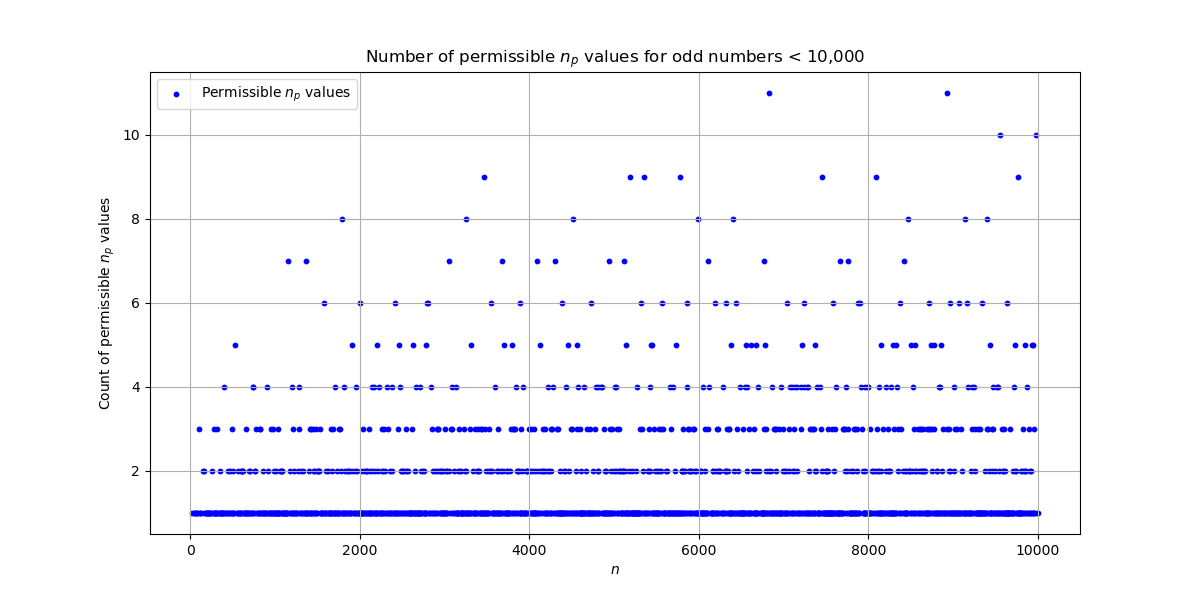
\includegraphics[width=0.75\linewidth]{exercise 4.5.47.png}
\begin{figure}[htbp]
    
    \begin{subfigure}{0.5\textwidth}
        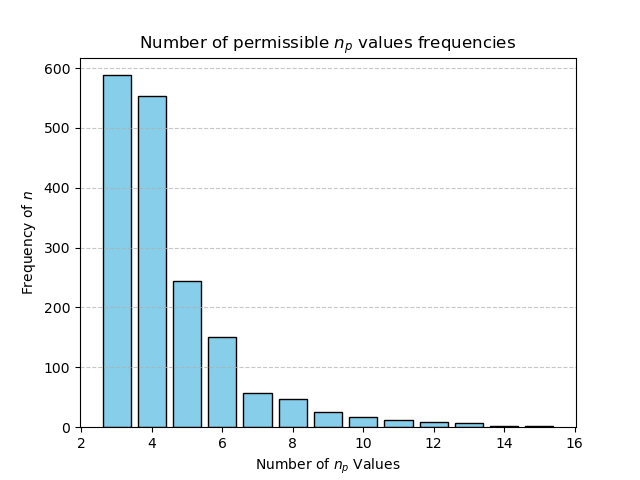
\includegraphics[width=\linewidth]{picture/exercise 4.5.47-2.png}
 \end{subfigure}
 \begin{subfigure}{0.5\textwidth}
        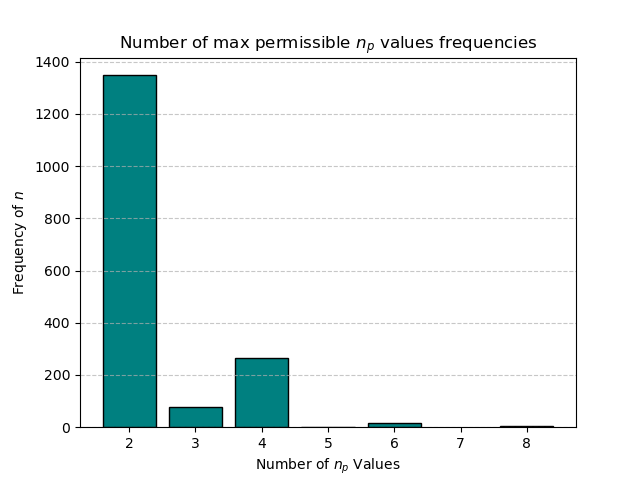
\includegraphics[width=\linewidth]{picture/exercise 4.5.47-3.png}
 \end{subfigure}
\end{figure}
\end{center}


\end{proof}
\begin{problem}{48}
    Carry out the same process as in the preceding exercise for all even numbers less than 1000. Explain the relative lengths of the lists versus the number of integers tested.
\end{problem}
\begin{proof}
    Similar to \textbf{Problem 47.}, you can run \texttt{Sylow.py} in 
    \begin{center}
        \texttt{\url{https://github.com/Laplacian2004/Dummit-Foote-sol/tree/main/code}}
    \end{center}
    with upper bound $100$, lower bound $2$, and step $2$, it will generate some figures and it will output the list in \texttt{np\_list.out}. Read the \texttt{Makefile} for some detailed instructions. Here are some results:
\begin{center}
        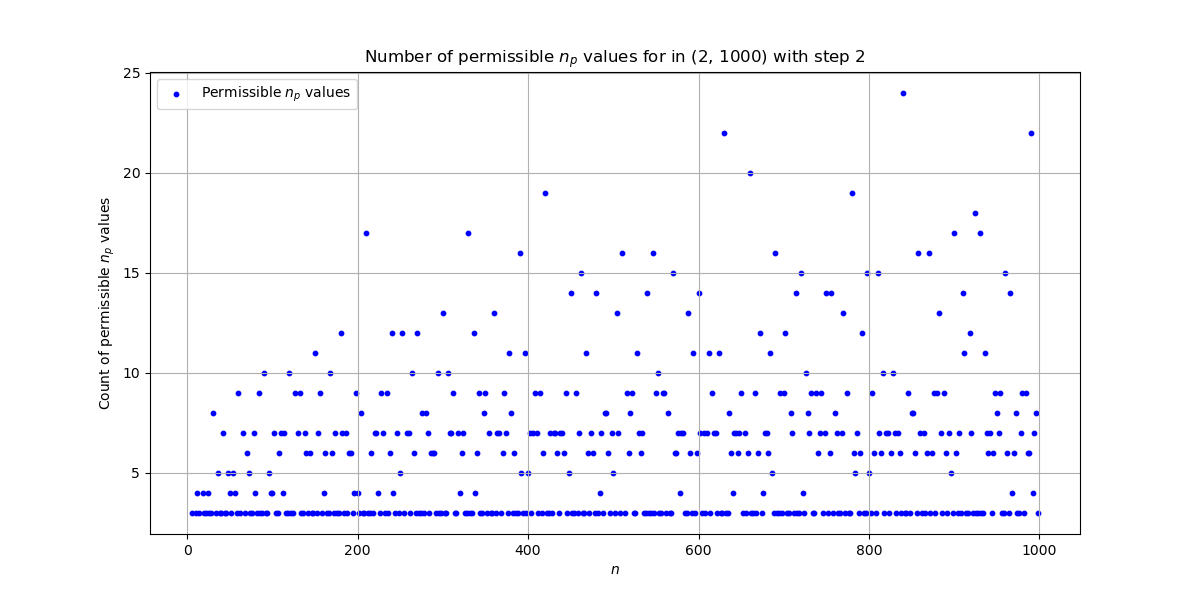
\includegraphics[width=0.75\linewidth]{picture/exercise 4.5.48.png}
\begin{figure}[htbp]
    
    \begin{subfigure}{0.5\textwidth}
        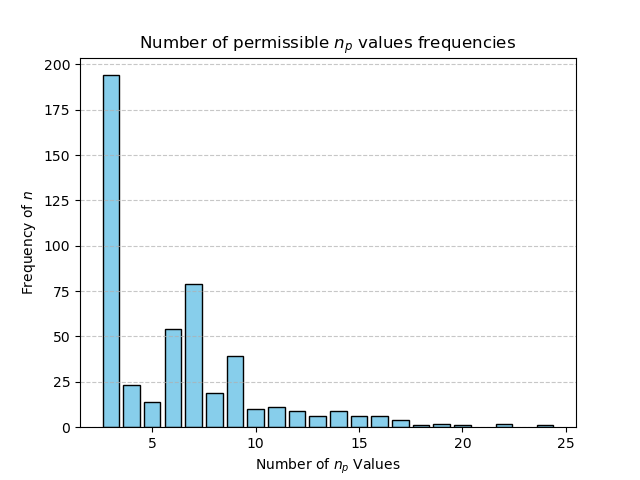
\includegraphics[width=\linewidth]{picture/exercise 4.5.48-2.png}
 \end{subfigure}
 \begin{subfigure}{0.5\textwidth}
        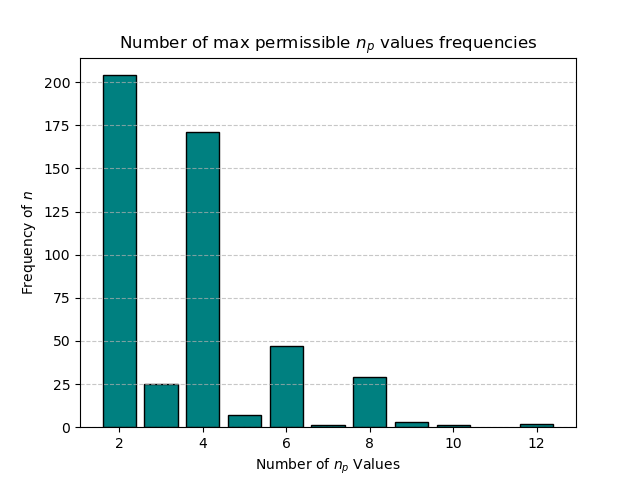
\includegraphics[width=\linewidth]{picture/exercise 4.5.48-3.png}
 \end{subfigure}
\end{figure}
\end{center}
\end{proof}
\begin{problem}{49}
    Prove that if $|G| = 2^m m$ where $m$ is odd and $G$ has a cyclic Sylow 2-subgroup then $G$ has a normal subgroup of order $m$. [Use induction and Exercises 11 and 12 in Section 2.]
\end{problem}
\begin{proof}
    We shall prove it by induction on $n$. When $n=1$, the statement has been proven in Exercises 11 and 12 in Section 2. Suppose that a normal subgroup of order $m$ exists for $n$ less than $k$. For $n$ equals $k$ since $G$ has a cyclic Sylow 2-subgroup, there exists element $x$ of order $2^n$, let $G$ acts on itself by left multiplication, let $\pi$ be the permutation presentation afford by this action, then $\pi(x)$ is the product of $m$ $2^n$-cycles, which is an odd permutation so that $\phi = \epsilon \circ \pi: G \rightarrow \{\pm 1\}$ is a surjective function. The first isomorphism theorem gives that 
    \[
        G/\ker(\phi) \cong Z_2
    \]
    then $|\ker(\phi)|=2^{n-1}m$, so by induction, there exist a order $m$ subgroup of $\ker(\phi)$, which is also a subgroup of $G$. 
\end{proof}
\begin{problem}{50}
        Prove that if $U$ and $W$ are normal subsets of a Sylow $p$-subgroup $P$ of $G$ then $U$ is conjugate to $W$ in $G$ if and only if $U$ is conjugate to $W$ in $N_G(P)$. Deduce that two elements in the center of $P$ are conjugate in $G$ if and only if they are conjugate in $N_G(P)$. 
    (A subset $U$ of $P$ is normal in $P$ if $N_P(U) = P$.)
\end{problem}
\begin{proof}
    Assumes that $P\in Syl_p(G)$ and $P=N_G(U)=N_G(W)$. Suppose $gUg^{-1}=W$ for some $g\in G$. Note that 
    \[
        gpg^{-1}W(gpg^{-1})^{-1}=gpg^{-1}gUg^{-1}(gpg^{-1})^{-1}=gUg^{-1}=W
    \]
    for all $p\in P$. Then $gPg^{-1}\leq N_G(W)=P$, and thus $g\in N_G(P)$. THerefore, $U$ is conjugates to $W$ in $N_G(P)$. The other direction is trivial, given that $N_G(P)\leq G$.\\
    Let $x, y\in Z(P)$, let $X=\{x\}$ and $Y=\{y\}$, note that $X$ and $Y$ are normal by definition. Suppose $x$, $y$ are conjugates in $G$, i.e. $X$, $Y$ is congugates in $G$, apply previous result on $X$ and $Y$ deduce that $X$ and $Y$ are congugates in $N_G(P)$, i.e. $x$ and $y$ are congugates in $N_G(P)$. The other direction is trivial, given that $N_G(P)\leq G$.
\end{proof}
\begin{problem}{51}
    Let $P$ be a Sylow $p$-subgroup of $G$ and let $M$ be any subgroup of $G$ which contains $N_G(P)$. Prove that $|G : M| \equiv 1 \pmod{p}$.
\end{problem}
\begin{proof}
    Since $P\in Syl_p(G)$, and $P\leq N_G(P)\leq M$, then we have that $P\in Syl_p(M)$. Since \[|G:M||M:N_G(P)|=|G:N_G(P)|=n_p(G)\], and $|M:N_G(P)|=|M:N_G(P)\cap M|=|M:N_M(P)|=n_p(M)$, so that 
    \[
        |G:M|n_p(M)=n_p(G)
    \]
    By Sylow's theorem, since $n_p(M)\equiv 1 \pmod p$ and $n_p(G) \equiv 1 \pmod p$, then $|G:M| \equiv 1 \pmod p$.
\end{proof}
\begin{problem}{52}
    Suppose $G$ is a finite simple group in which every proper subgroup is abelian. 
    If $M$ and $N$ are distinct maximal subgroups of $G$, prove $M \cap N = 1$. 
    [See Exercise 23 in Section 3.]
\end{problem}
\begin{proof}
    Assume that $G$ is a finite simple group in which every proper subgroup is abelian. Let $N$ and $M$ be distinct maximal subgroups in $G$. Suppose $N\cap M$ is non-trivial. Since $G$ is simple, then $N_G(N\cap M)\neq G$. Since $M$ and $N$ are abelian subgroup then $N, M\leq N_G(N\cap M)$, so that the maximality of $N$ and $M$ forces $N_G(N\cap M)=N=M$, contradicts the fact that $N$ and $M$ are distinct. Therefore, $N\cap M=1$
\end{proof}
\begin{problem}{53}
    Use the preceding exercise to prove that if $G$ is any non-abelian group in which every proper subgroup is abelian, then $G$ is not simple. 
    [Let $G$ be a counterexample to this assertion and use Exercise 24 in Section 3 to show that $G$ has more than one conjugacy class of maximal subgroups. 
    Use the method of Exercise 23 in Section 3 to count the elements which lie in all conjugates of $M$ and $N$, where $M$ and $N$ are nonconjugate maximal subgroups of $G$; 
    show that this gives more than $|G|$ elements.]
\end{problem}
\begin{proof}
    By way of contradiction, suppose $G$ be a non-abelian simple group in which every proper subgroup is abelian. We first claim that there exists maximal subgroup such that they are not in the same conjugacy class. Suppose that every maximal subgroup is conjugate to another. Let $M$ be an arbitrary maximal subgroup in $G$. For any $x \in G$, let $M_x$ be the maximal subgroup containing $x$, then $M_x = gMg^{-1}$. Since 
    \[
        G=\bigcup_{x\in G}M_x \leq \bigcup_{g\in G}gMg^{-1} \leq G
    \]
    then $G=\bigcup_{g\in G}gMg^{-1}$, contradicting Exercise 24 in Section 3. Let $M$ and $N$ be two distinct maximal subgroups in $G$ such that they are not in the same conjugacy class. Since $gMg^{-1}=hMh^{-1}$ if and only if $g M=hM$, then there are exactly $|G:M|$ in the conjugacy class of $M$. Suppose $gMg^{-1}<H<G$ then 
    $M<g^{-1}Hg<G$, which is not possible, then $gMg^{-1}$ is also maximal. Since the intersection of distinct maximal subgroups is $1$, then 
    \[
        |G|>|G:M|(|M|-1)+|G:N|(|N|-1)\geq \frac{|G|}{2}+\frac{|G|}{2}=|G|
    \]
    which is a contradiction. Therefore, $G$ can not be simple.
\end{proof}
\begin{problem}{54}
    Prove the following classification: if $G$ is a finite group of order $p_1 p_2 \cdots p_r$, where the $p_i$'s are distinct primes such that $p_i$ does not divide $p_j - 1$ for all $i$ and $j$, 
    then $G$ is cyclic. 
    [By induction, every proper subgroup of $G$ is cyclic, so $G$ is not simple by the preceding exercise. 
    If $N$ is a nontrivial proper normal subgroup, $N$ is cyclic, and $G/N$ acts as automorphisms of $N$. 
    Use Proposition 16 to show that $N \leq Z(G)$ and use induction to show $G/Z(G)$ is cyclic, hence $G$ is abelian by Exercise 36 of Section 3.1.]
\end{problem}
\begin{proof}
    We show the statement by doing induction on $r$. For $r=1$, since $|G|=p_1$, then $G\cong Z_{p_1}$, and is cyclic. Suppose for $r<k$ the statement is true. For $r=k$, since every subgroup of $G$ is cyclic by induction, then $G$ is not simple by the previous exercise. Let $N$ be a nontrivial normal subgroup in $G$, then $G$ is cyclic by induction. Since $N$ is normal let $G$ acts on $N$ by conjugation, then 
    \[
        G/C_G(N) \xhookrightarrow{} \Aut(N) \cong (\Z/n\Z)^{\times}
    \]
    where $n=|N|$. Since $|H|=p_{n_1}\dots p_{n_m}$ where $n_i\in \{1, \dots r\}$ and $n_i\neq n_j$ for $i\neq j$, then $|(\Z/n\Z)^{\times}|=(p_{n_1}-1)\dots (p_{n_m}-1)$. Since no $p_j$ divides $p_{n_i}-1$ where $j\in \{1, \dots r\} \setminus \{n_1, \dots ,n_m\}$ and $N\leq C_G(N)$ so that there is no factor of $p_{n_i}$ in $|G/C_G(N)|$, then we immediately have $|G/C_G(N)|=1$, i.e. $G=C_G(N)$ or $N\leq Z(G)$. Since $N$ is non-trivial, $Z(G)\neq 1$ so that $G/Z(G)$ is cyclic by induction; hence, $G$ is abelian. Cauchy theorem gives that there exist elements $x_i$ with order $p_i$ for each $i\in \{1, ..., r\}$. Since $x_1\cdots x_r$ is element of order $p_1\dots p_r$, then $G$ is cyclic. This completes the proof.
\end{proof}
\begin{problem}{55}
     Prove the converse to the preceding exercise: if $n \geq 2$ is an integer such that every group of order $n$ is cyclic, 
    then $n = p_1 p_2 \cdots p_r$ is a product of distinct primes and $p_i$ does not divide $p_j - 1$ for all $i, j$. 
    [If $n$ is not of this form, construct noncyclic groups of order $n$ using direct products of noncyclic groups of order $p^2$ and $pq$, where $p \mid q - 1$.]
\end{problem}
\begin{proof}
    Let $G$ be a cyclic subgroup of order $n$. By way of contradiction, suppose that $n$ is not a product of distinct prime or $p_i \mid p_j-1$ for some $i, j$.
    If $n$ is not a product of distinct prime i.e there exists $p_i = p_j$ for some $i\neq j$, then construct a group $G$ such that 
    \[
        G=\langle a \rangle \times \langle b \rangle \times \langle c \rangle\simeq Z_{p_i}\times Z_{p_i} \times Z_m
    \]
    where $n=mp_i^2$. Note that $|G|=p_i^2m=n$ and since for every $x\in G$, write $x =a^ib^ic^j$, $x^{pm}=1$, then there is no order $mp_i^2$ element in $G$ and hence $G$ is not cyclic, which is a contradiction.
    Otherwise suppose $n=p_1\dots p_r$ and $p_i\mid p_j-1$ for some $i, j$. Construct a group $G$ such that 
    \[
        G=M\times Z_m
    \]
    where $n=mp_ip_j$ and $M$ obtained by first let $P=\langle x \rangle\in Syl_{p_j}(S_{p_j})$ and since $|N_{S_{p_j}}(P)|=p_j(p_j-1)$, by Cauchy theorem, there exists a subgroup $Q=\langle y \rangle$ of order $p_i$ and $QP$ is a group of order $p_ip_j$, and take $M=QP$. Note that $M$ is non-abelian since $C_{S_{p_j}}(P)=P$, so that $(x, 1)$ does not commute with $(y, 1)$. Therefore, $G$ is a non-abelian subgroup of order $|G|=p_ip_jm=n$, thus $G$ is not cyclic, which is a contradiction.
\end{proof}
\begin{problem}{56}
         If $G$ is a finite group in which every proper subgroup is abelian, show that $G$ is solvable.
\end{problem}
\begin{proof}
    We shall induct on the order of $|G|$. For $|G|=1$, the statement is trivial. 
    Suppose $G$ is abelian, then $1 \trianglelefteq G$ is trivially a normal tower so that $G$ is solvable. Suppose $G$ is non-abelian, then \textbf{Exercise 53} shows that $G$ is not simple so that there exists proper nontrivial normal subgroup $N$ of $G$, and $N$ is abelian by assumption. Let $H/N=\overline{H}< G/N$, since the preimage $H$ is abelian, then $H/N$ is also abelian, so that every subgroup of $G/N$ is then abelian. Since $|G/N|<|G|$, induction shows that there exists an abelian normal tower $\{M_i\}$ such that 
    \[M_1=\overline{1}\trianglelefteq \cdots \trianglelefteq G/N=M_k\]
    of $G/N$. Let $N_i$ be the preimage of $M_i=N_i/N$ under the canonical homomorphism, and Lattice isomorphism gives that 
    \[
        N_1=N\trianglelefteq \cdots \trianglelefteq G=N_k
    \]
    Since $N_1=N$ is abelian by assumption, then $\{N_i\}$ is a normal abelian tower in $G$, and thus $G$ is solvable.
\end{proof}
\section*{4.6 The Simplicity of $A_n$}
Missing exercise number : 8
\begin{problem}{1}
 Prove that $A_n$ does not have a proper subgroup of index $< n$ for all $n \geq 5$.
\end{problem}
\begin{proof}
    Suppose that $H$ is a subgroup such that $m=|A_n:H|<n$. Let $A_n$ act on the set of left cosets of $H$ by left multiplication, and $\varphi$ is the homomorphism afforded by this action. Since $A_n$ is simple for $n\geq 5$ and $\ker \varphi =\cap_{g \in G} g Hg^{-1}\leq H$, then we have that $\ker \varphi=1$. Then 
    \[
         A_n \xhookrightarrow{\varphi} S_m
    \]
    but since $m!\leq (n-1)!=\frac{n!}{n}< n!/2$ since $n\geq 5$, then $\varphi(A_n)$ cannot be a subgroup of $S_m$, contradict with the fact that $\varphi$ is injective.
\end{proof}
\begin{problem}{2}
     Find all normal subgroups of $S_n$ for all $n \geq 5$.
\end{problem}
\begin{proof}
    Suppose that $N$ is a non-trivial proper normal subgroup of $S_n$ for $n\geq 5$. Let $M=A_n\cap N$ is normal, since $A_n$ is simple, $M=A_n$ or $M=1$. If $M=A_n$, then $A_n\leq N$, but since $A_n$ has index 2, one must have $N=A_n$. If $M=1$, then $N\neq A_n$, and by second isomorphism theorem, 
    \[
        S_n/N = NA_n/N \cong A_n/(A_n \cap N)
    \]
    which gives that $|N|=2$. then $N=\langle \sigma \rangle$ where $\sigma$ is tranpositions. But since transpositions are conjugates with each other, $N$ is not normal.\\
    It is possible to show since $S_n'=A_n$, and $[S_n, N]\leq N\cap S_n'=M=1$, then $N\leq Z(S_n)=1$.
    Therefore, the only possible normal groups for $S_n$ are $\{1, A_n, S_n\}$ for all $n\geq 5$.
\end{proof}
\begin{problem}{3}
    Prove that $A_n$ is the only proper subgroup of index $< n$ in $S_n$ for all $n \geq 5$.
\end{problem}
\begin{proof}
    Let $H$ be a proper subgroup such that $m=|S_n:H|<n$. Let $G$ act on the set of left cosets of $H$ by conjugation, and let $\varphi$ be the permutation presentation afforded by this action, then 
    \[
        \varphi : S_n \rightarrow S_m 
    \]
    . Since $n>m$, then $\ker \varphi \neq 1 $ and since $\ker \varphi \leq H$, then $\ker \varphi <G$. But previous exercise show that the only normal subgroup of $S_n$ is $A_n$, and therefore $\ker\phi =A_n$. Since $A_n =\ker \varphi \leq H \leq G$, then $H=A_n$.   
\end{proof}
\begin{problem}{4}
        Prove that $A_n$ is generated by the set of all 3-cycles for each $n \geq 3$.
\end{problem}
\begin{proof}
    Let $\sigma \in A_n$. Write $\sigma = \lambda_1 \dots \lambda_{2t}$ where $\lambda$ is transposition in $S_n$. It suffices to show that a product of two transpositions can be written as 
    a product of $3$-cycles.
    \begin{enumerate}[1.]
        \item If two transpositions $\tau=(a\, b), \gamma =(c\, d)$ are disjoint (implictly, $n\geq 4$), then 
        \[
            (a\, b)(c\, d)=(a\, b)(b\, c)(b\, c)(c\, d)=(b\, c\, a)(c\, d\, b)
        \]
        \item If two transpositions $\tau=(a\, b), \gamma =(a\, c)$ intersect one element, then 
        \[
            (a\, b)(a\, c)=(a\, c\, b)
        \]
        \item If two transpositions are the same, then
        \[
            (a\, b)(a\, b)=1
        \]
    \end{enumerate}
    Therefore, every element in $A_n$ is generated by $3$-cycles for $n\geq 3$.
\end{proof}
\begin{problem}{5}
        Prove that if there exists a chain of subgroups $G_1 \leq G_2 \leq \cdots \leq G$ such that $G = \bigcup_{i=1}^{\infty} G_i$ and each $G_i$ is simple, then $G$ is simple.
\end{problem}
\begin{proof}
    When $|G|=1$ the statement is trivial. Assume that $|G|\neq 1$. Suppose $N$ is a normal subgroup of $G$, then 
    \[
        N=G\cap N = \cup_{i=1}^\infty (G_i\cap N)
    \]
    Since $(G_i\cap N) \trianglelefteq  G_i$, simplicity of $G_i$ forces $G_i\cap N=1$ or $G_i\cap N=G_i$. Suppose $G_i\cap N\neq 1$ for some $i$, then $G_i\leq N$ so that $G_i\leq N\cap G_j$ for $j\geq i$. Since $G_i\neq 1$, then $N\cap G_j\neq 1$ so that $N\cap G_j=G_j$ for $j\geq i$, and it follows that $G\leq N$ and thus $N=G$. Suppose $G_i\cap N=1$ for all $i$, then $N=1$. Therefore, $G$ is simple.
\end{proof}
\begin{problem}{6}
         Let $D$ be the subgroup of $S_\Omega$ consisting of permutations which move only a finite number of elements of $\Omega$ (described in Exercise 17 in Section 3), and let $A$ be the set of all elements $\sigma \in D$ such that $\sigma$ acts as an even permutation on the (finite) set of points it moves. 
    Prove that $A$ is an infinite simple group. 
    [Show that every pair of elements of $D$ lie in a finite simple subgroup of $D$.]
\end{problem}
\begin{proof}
    Let $\tau, \sigma \in A$. Since $\tau\sigma^{-1}$ fix finite number of points and $\tau \sigma^{-1}$ is even, then $\tau\sigma^{-1}\in A$, so $A$ is a group. Suppose $N$ is some non-trivial normal subgroup in $A$ with $\gamma\in N-\{1\}$, and let $\Delta\subseteq \Omega$ be the set move either by $\tau$ or $\gamma$. If $|\Delta|<5$ append elements in $\Omega$ so that $|\Delta|=5$. Let $H$ be a subgroup of $D$ such that it fixed all points in $\Omega\setminus \Delta$, then $H\cong A_{\Delta}$. Since $\gamma, \tau\in H$ and $\gamma\in N$, then $H\cap N \trianglelefteq H$, and simplicity of $H$ forces $H\cap N = H$, given that $1\neq \gamma\in H\cap N$. So since $\tau \in H$, then $\tau \in N$. Therefore, $A\leq N$ and thus $N=A$.
\end{proof}
\begin{problem}{7}
     Under the notation of the preceding exercise, prove that if $H \trianglelefteq S_\Omega$ and $H \neq 1$, then $A \leq H$, i.e., $A$ is the unique (nontrivial) minimal normal subgroup of $S_\Omega$.
\end{problem}
\begin{proof}
    Let $H\trianglelefteq S_{\Omega}$ and $H\neq 1$. Since $H\cap A\trianglelefteq A$, then simplicity of $A$ forces $H\cap A=1$ or $H\cap A=A$. For $H\cap A=A$, then $A\leq H$, we are done. For $H\cap A=1$, note that $A\trianglelefteq S_{\Omega}$ given by $D\trianglelefteq S_{\Omega}$ and $A_{\Omega}\trianglelefteq S_{\Omega}$, then $[H, A]\leq H\cap A =1$, then $H\leq C=C_{S_{\Omega}}(A)$. For all $a \in \Omega$, construct $(a\, b\, c)\in A_a$, note that $C$ commutes with $(a\, b\, c)$ for all $b, c\in \Omega\setminus \{a\}$ and hence have cycles that does not contain $a$. Therefore, $C=1$ and hence $H=1$ which is a contradiction. It follows that $A \leq H$, i.e., $A$ is the unique (nontrivial) minimal normal subgroup of $S_\Omega$.
\end{proof}
\begin{problem}{8}
    Under the notation of the preceding two exercises, prove that $|D| = |A| = |\Omega|$. Deduce that 
    \[
    \text{if } S_\Omega \cong S_\Delta, \text{ then } |\Omega| = |\Delta|.
    \]
    [Use the fact that $D$ is generated by transpositions. You may assume that countable unions and finite direct products of sets of cardinality $|\Omega|$ also have cardinality $|\Omega|$.]
\end{problem}
\begin{proof}
    
\end{proof}
\end{document}                                                                                                                           
